% Options for packages loaded elsewhere
\PassOptionsToPackage{unicode}{hyperref}
\PassOptionsToPackage{hyphens}{url}
%
\documentclass[
]{book}
\usepackage{lmodern}
\usepackage{amssymb,amsmath}
\usepackage{ifxetex,ifluatex}
\ifnum 0\ifxetex 1\fi\ifluatex 1\fi=0 % if pdftex
  \usepackage[T1]{fontenc}
  \usepackage[utf8]{inputenc}
  \usepackage{textcomp} % provide euro and other symbols
\else % if luatex or xetex
  \usepackage{unicode-math}
  \defaultfontfeatures{Scale=MatchLowercase}
  \defaultfontfeatures[\rmfamily]{Ligatures=TeX,Scale=1}
\fi
% Use upquote if available, for straight quotes in verbatim environments
\IfFileExists{upquote.sty}{\usepackage{upquote}}{}
\IfFileExists{microtype.sty}{% use microtype if available
  \usepackage[]{microtype}
  \UseMicrotypeSet[protrusion]{basicmath} % disable protrusion for tt fonts
}{}
\makeatletter
\@ifundefined{KOMAClassName}{% if non-KOMA class
  \IfFileExists{parskip.sty}{%
    \usepackage{parskip}
  }{% else
    \setlength{\parindent}{0pt}
    \setlength{\parskip}{6pt plus 2pt minus 1pt}}
}{% if KOMA class
  \KOMAoptions{parskip=half}}
\makeatother
\usepackage{xcolor}
\IfFileExists{xurl.sty}{\usepackage{xurl}}{} % add URL line breaks if available
\IfFileExists{bookmark.sty}{\usepackage{bookmark}}{\usepackage{hyperref}}
\hypersetup{
  pdftitle={SingleCell Workshop},
  pdfauthor={Yuanhua lab},
  hidelinks,
  pdfcreator={LaTeX via pandoc}}
\urlstyle{same} % disable monospaced font for URLs
\usepackage{color}
\usepackage{fancyvrb}
\newcommand{\VerbBar}{|}
\newcommand{\VERB}{\Verb[commandchars=\\\{\}]}
\DefineVerbatimEnvironment{Highlighting}{Verbatim}{commandchars=\\\{\}}
% Add ',fontsize=\small' for more characters per line
\usepackage{framed}
\definecolor{shadecolor}{RGB}{248,248,248}
\newenvironment{Shaded}{\begin{snugshade}}{\end{snugshade}}
\newcommand{\AlertTok}[1]{\textcolor[rgb]{0.94,0.16,0.16}{#1}}
\newcommand{\AnnotationTok}[1]{\textcolor[rgb]{0.56,0.35,0.01}{\textbf{\textit{#1}}}}
\newcommand{\AttributeTok}[1]{\textcolor[rgb]{0.77,0.63,0.00}{#1}}
\newcommand{\BaseNTok}[1]{\textcolor[rgb]{0.00,0.00,0.81}{#1}}
\newcommand{\BuiltInTok}[1]{#1}
\newcommand{\CharTok}[1]{\textcolor[rgb]{0.31,0.60,0.02}{#1}}
\newcommand{\CommentTok}[1]{\textcolor[rgb]{0.56,0.35,0.01}{\textit{#1}}}
\newcommand{\CommentVarTok}[1]{\textcolor[rgb]{0.56,0.35,0.01}{\textbf{\textit{#1}}}}
\newcommand{\ConstantTok}[1]{\textcolor[rgb]{0.00,0.00,0.00}{#1}}
\newcommand{\ControlFlowTok}[1]{\textcolor[rgb]{0.13,0.29,0.53}{\textbf{#1}}}
\newcommand{\DataTypeTok}[1]{\textcolor[rgb]{0.13,0.29,0.53}{#1}}
\newcommand{\DecValTok}[1]{\textcolor[rgb]{0.00,0.00,0.81}{#1}}
\newcommand{\DocumentationTok}[1]{\textcolor[rgb]{0.56,0.35,0.01}{\textbf{\textit{#1}}}}
\newcommand{\ErrorTok}[1]{\textcolor[rgb]{0.64,0.00,0.00}{\textbf{#1}}}
\newcommand{\ExtensionTok}[1]{#1}
\newcommand{\FloatTok}[1]{\textcolor[rgb]{0.00,0.00,0.81}{#1}}
\newcommand{\FunctionTok}[1]{\textcolor[rgb]{0.00,0.00,0.00}{#1}}
\newcommand{\ImportTok}[1]{#1}
\newcommand{\InformationTok}[1]{\textcolor[rgb]{0.56,0.35,0.01}{\textbf{\textit{#1}}}}
\newcommand{\KeywordTok}[1]{\textcolor[rgb]{0.13,0.29,0.53}{\textbf{#1}}}
\newcommand{\NormalTok}[1]{#1}
\newcommand{\OperatorTok}[1]{\textcolor[rgb]{0.81,0.36,0.00}{\textbf{#1}}}
\newcommand{\OtherTok}[1]{\textcolor[rgb]{0.56,0.35,0.01}{#1}}
\newcommand{\PreprocessorTok}[1]{\textcolor[rgb]{0.56,0.35,0.01}{\textit{#1}}}
\newcommand{\RegionMarkerTok}[1]{#1}
\newcommand{\SpecialCharTok}[1]{\textcolor[rgb]{0.00,0.00,0.00}{#1}}
\newcommand{\SpecialStringTok}[1]{\textcolor[rgb]{0.31,0.60,0.02}{#1}}
\newcommand{\StringTok}[1]{\textcolor[rgb]{0.31,0.60,0.02}{#1}}
\newcommand{\VariableTok}[1]{\textcolor[rgb]{0.00,0.00,0.00}{#1}}
\newcommand{\VerbatimStringTok}[1]{\textcolor[rgb]{0.31,0.60,0.02}{#1}}
\newcommand{\WarningTok}[1]{\textcolor[rgb]{0.56,0.35,0.01}{\textbf{\textit{#1}}}}
\usepackage{longtable,booktabs}
% Correct order of tables after \paragraph or \subparagraph
\usepackage{etoolbox}
\makeatletter
\patchcmd\longtable{\par}{\if@noskipsec\mbox{}\fi\par}{}{}
\makeatother
% Allow footnotes in longtable head/foot
\IfFileExists{footnotehyper.sty}{\usepackage{footnotehyper}}{\usepackage{footnote}}
\makesavenoteenv{longtable}
\usepackage{graphicx}
\makeatletter
\def\maxwidth{\ifdim\Gin@nat@width>\linewidth\linewidth\else\Gin@nat@width\fi}
\def\maxheight{\ifdim\Gin@nat@height>\textheight\textheight\else\Gin@nat@height\fi}
\makeatother
% Scale images if necessary, so that they will not overflow the page
% margins by default, and it is still possible to overwrite the defaults
% using explicit options in \includegraphics[width, height, ...]{}
\setkeys{Gin}{width=\maxwidth,height=\maxheight,keepaspectratio}
% Set default figure placement to htbp
\makeatletter
\def\fps@figure{htbp}
\makeatother
\setlength{\emergencystretch}{3em} % prevent overfull lines
\providecommand{\tightlist}{%
  \setlength{\itemsep}{0pt}\setlength{\parskip}{0pt}}
\setcounter{secnumdepth}{5}
\usepackage{booktabs}
\usepackage[]{natbib}
\bibliographystyle{apalike}

\title{SingleCell Workshop}
\author{Yuanhua lab}
\date{2021-07-02}

\begin{document}
\maketitle

{
\setcounter{tocdepth}{1}
\tableofcontents
}
\hypertarget{introduction}{%
\chapter{Introduction}\label{introduction}}

\textbf{Cell interaction and Cell differentiation trajectory}

\begin{itemize}
\tightlist
\item
  Cell interaction with ligand and receptors
\item
  Pseudo-time and trajectory analysis
\item
  RNA velocity
\end{itemize}

\textbf{Cellular genetics}

\begin{itemize}
\tightlist
\item
  mtDNA variants for lineage inference from single-cell omics
\item
  Copy number variation estimation from scRNA-seq
\item
  Nuclear SNV analysis in single-cell omics
\end{itemize}

\hypertarget{env-pre}{%
\chapter{Prerequisites}\label{env-pre}}

\hypertarget{wsl_install}{%
\section{(Optional) Install Windows Subsystem for Linux}\label{wsl_install}}

\textbf{Note, this is for Windows users only.} While some required softwares only support Linux or macOS, you could install WSL to use Linux inside Windows.

If you already have Linux or macOS, you can skip this section and jump directly to the section of \texttt{conda\ installation} \protect\hyperlink{conda_install_linux}{for Linux} or \protect\hyperlink{conda_install_mac}{for macOS}.

The whole process of installing WSL requires at least 2G disk space. Note that this process was tested on Windows 10 (Version 2004, build 19041.1052).

\hypertarget{what-is-the-windows-subsystem-for-linux-wsl}{%
\subsection{What is the Windows Subsystem for Linux (WSL)?}\label{what-is-the-windows-subsystem-for-linux-wsl}}

According to the \href{https://docs.microsoft.com/en-us/windows/wsl/about}{Microsoft Docs},

\begin{quote}
\emph{``The Windows Subsystem for Linux lets developers run a GNU/Linux environment -- including most command-line tools, utilities, and applications -- directly on Windows, unmodified, without the overhead of a traditional virtual machine or dualboot setup.''}
\end{quote}

\hypertarget{manual-installation-steps}{%
\subsection{Manual Installation Steps}\label{manual-installation-steps}}

\textbf{Step 1. Enable required feature in Windows PowerShell}

It is necessary to enable the required feature for WSL before installing it.

\begin{itemize}
\tightlist
\item
  Type \texttt{powershell} in the search box of the Windows taskbar.
\item
  Right click \texttt{Windows\ PowerShell} and select \texttt{Run\ as\ administrator}.
\end{itemize}

\begin{center}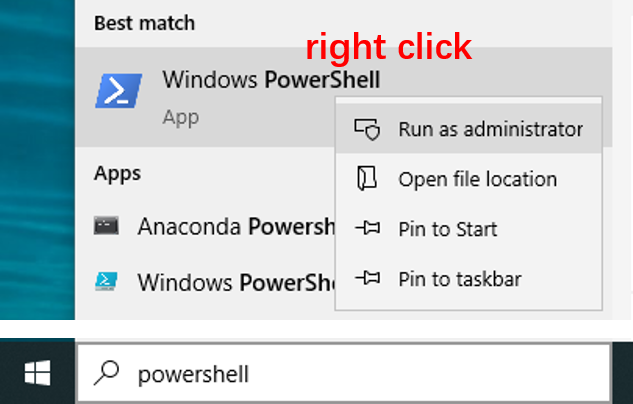
\includegraphics[width=0.45\linewidth]{./images/wsl_open_powershell} \end{center}

\begin{itemize}
\tightlist
\item
  Type the command below in PowerShell.
\end{itemize}

\begin{verbatim}
dism.exe /online /enable-feature /featurename:Microsoft-Windows-Subsystem-Linux /all /norestart
\end{verbatim}

\begin{center}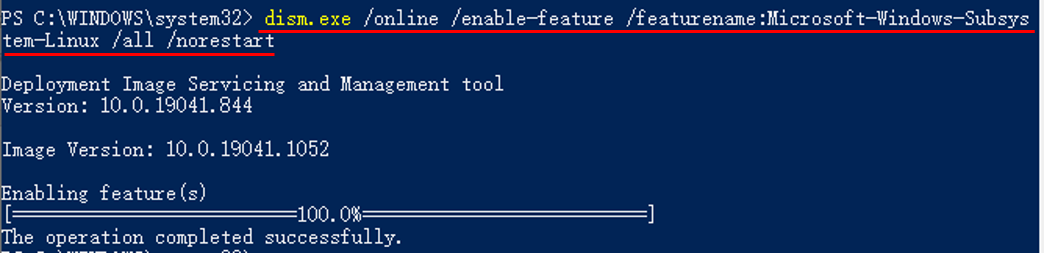
\includegraphics[width=0.6\linewidth]{./images/wsl_enable_feature} \end{center}

\textbf{Step 2. Download and install WSL}

Microsoft now supports several Linux distributions as WSL, such as Ubuntu, openSUSE, Fedora, etc (\href{https://docs.microsoft.com/en-us/windows/wsl/install-win10\#step-6---install-your-linux-distribution-of-choice}{a full list here}), among which we choose Ubuntu as an example.

Ubuntu WSL could be freely downloaded and installed through \href{https://www.microsoft.com/en-us/p/ubuntu-2004-lts/9n6svws3rx71?rtc=1\&activetab=pivot:overviewtab}{Microsoft Store}.

\begin{itemize}
\tightlist
\item
  Go to the webpage for \href{https://www.microsoft.com/en-us/p/ubuntu-2004-lts/9n6svws3rx71?rtc=1\&activetab=pivot:overviewtab}{Ubuntu} in Microsoft Store.
\item
  Click on the \texttt{Get} button.
\item
  Wait for completion of downloading and installation.
\item
  Click on the \texttt{Launch} button.
\end{itemize}

\begin{center}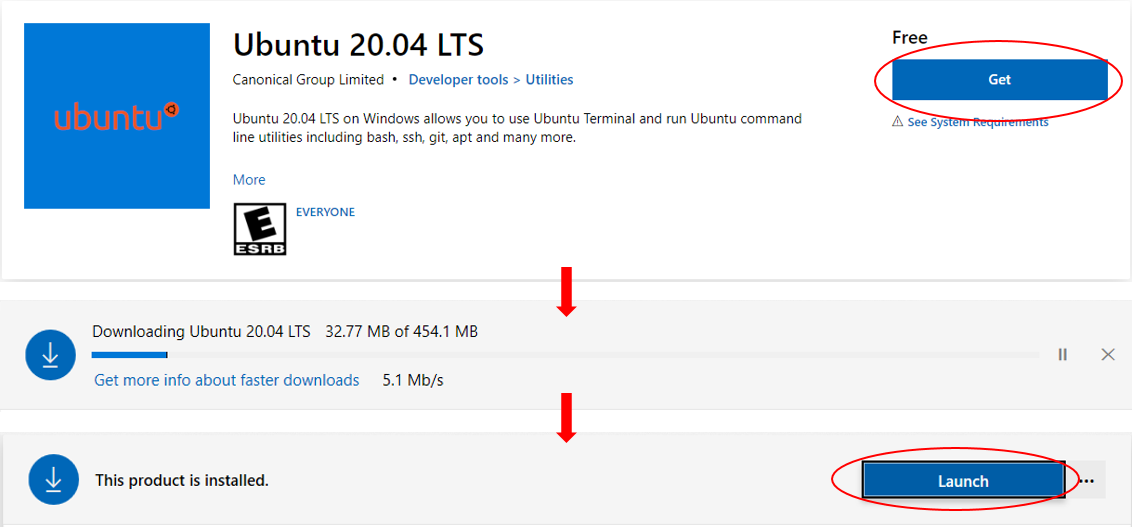
\includegraphics[width=0.6\linewidth]{./images/wsl_download_install} \end{center}

\textbf{Step 3. Create a new account for Ubuntu}

After successfully installing Ubuntu, a new user account should be created.

\begin{itemize}
\tightlist
\item
  Type user name and password following the prompts on the screen. Note, it is normal that the password is invisible when you are typing.
\end{itemize}

\begin{center}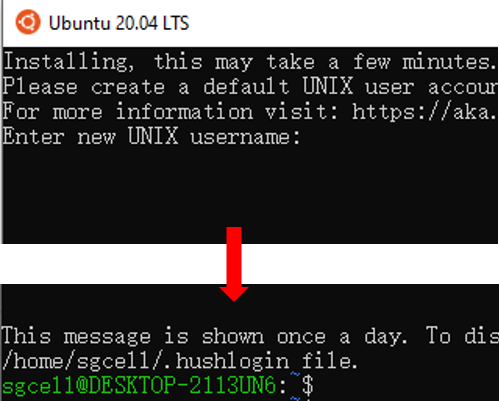
\includegraphics[width=0.4\linewidth]{./images/wsl_create_account} \end{center}

\textbf{Now Congratulations! You have successfully installed and set up Ubuntu in your Windows System!}

Next time you can re-open Ubuntu through the search box of the Windows taskbar.

\begin{center}
\includegraphics[width=0.35\linewidth]{./images/wsl_open_ubuntu} \end{center}

More information about the usage of WSL can be found at \href{https://docs.microsoft.com/en-us/windows/wsl}{Microsoft Docs}.

\hypertarget{conda_install}{%
\section{Install Conda Environment}\label{conda_install}}

The whole process of installing conda environment requires at least 1G disk space.

\hypertarget{what-is-conda}{%
\subsection{What is conda?}\label{what-is-conda}}

Conda is part of the Anaconda platform. According to the \href{https://docs.anaconda.com/\#anaconda-individual-edition}{Anaconda docs},

\begin{quote}
\emph{``Anaconda Individual Edition is a free, easy-to-install package manager, environment manager, and Python distribution with a collection of 1,500+ open source packages with free community support. Anaconda is platform-agnostic, so you can use it whether you are on Windows, macOS, or Linux.''}
\end{quote}

For quick installation and configuration, we choose to install \href{https://docs.conda.io/en/latest/miniconda.html}{Miniconda} instead of the whole Anaconda.

\begin{quote}
\emph{``Miniconda is a free minimal installer for conda. It is a small, bootstrap version of Anaconda that includes only conda, Python, the packages they depend on, and a small number of other useful packages, including pip, zlib and a few others.''}
\end{quote}

\hypertarget{conda_install_windows}{%
\subsection{Installation on Windows}\label{conda_install_windows}}

Although it is easy to install Miniconda itself on Windows, there are several conda softwares (e.g., bcftools, cellsnp-lite) required for this workshop that are well-supported only on Unix-Like systems. Linux or macOS is essential to use those softwares.

Good news is that Microsoft has provided the Windows Subsystem for Linux (WSL), which enables you to use several Linux distributions on Windows 10. The installation of WSL is easy and details can be found \protect\hyperlink{wsl_install}{here}.

After installing WSL, you could follow Section \protect\hyperlink{conda_install_linux}{Installation on Linux} to install Miniconda on WSL.

\hypertarget{conda_install_linux}{%
\subsection{Installation on Linux}\label{conda_install_linux}}

This section is adapted based on Miniconda installation \href{https://conda.io/projects/conda/en/latest/user-guide/install/linux.html}{guides for Linux}. In this section, we select the Miniconda with Python 3.9 as an example.

\textbf{Step 1. Open Shell}

\begin{itemize}
\tightlist
\item
  Open Linux Shell / WSL Shell (see Section \protect\hyperlink{wsl_install}{Install WSL} for details of WSL).
\end{itemize}

\textbf{Step 2. Download Miniconda installer}

The Miniconda installer is a \texttt{.sh} file containing metadata of installation. Run \texttt{wget\ \textless{}installer\_link\textgreater{}} to download the installer. e.g.,

\begin{itemize}
\tightlist
\item
  Type in Shell \texttt{wget\ https://repo.anaconda.com/miniconda/Miniconda3-py39\_4.9.2-Linux-x86\_64.sh}.
\end{itemize}

\begin{center}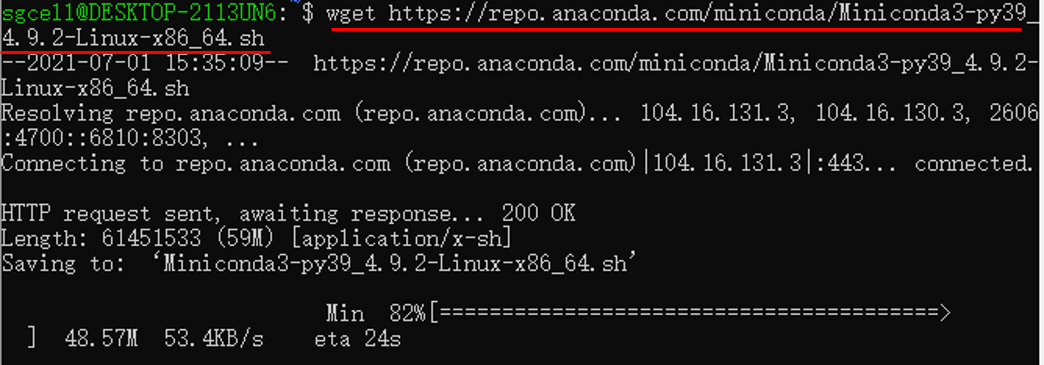
\includegraphics[width=0.65\linewidth]{./images/conda_download_installer} \end{center}

You could choose other Miniconda installers based on your platform. A full list of installers can be found \href{https://docs.conda.io/en/latest/miniconda.html}{here}.

\textbf{Step 3. Verify your installer hashes (Optional)}

An unmatched hash indicates there were some error during the downloading process. We could simply verify the installer hashes by typing \texttt{sha256sum\ \textless{}installer\_file\textgreater{}} in the Shell. e.g.,

\begin{itemize}
\tightlist
\item
  Type \texttt{sha256sum\ Miniconda3-py39\_4.9.2-Linux-x86\_64.sh} and check if the output hash is \texttt{536817d1b14cb1ada88900f5be51ce0a5e042bae178b5550e62f61e223deae7c}.
\end{itemize}

\begin{center}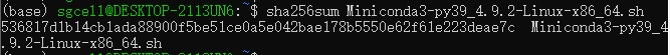
\includegraphics[width=0.65\linewidth]{./images/conda_verify_hash} \end{center}

A full list of hashes can be found \href{https://docs.conda.io/en/latest/miniconda.html}{here}.

\textbf{Step 4. Initialize Miniconda}

Run \texttt{bash\ \textless{}installer\_file\textgreater{}} in Shell. e.g.,

\begin{itemize}
\tightlist
\item
  Type \texttt{bash\ Miniconda3-py39\_4.9.2-Linux-x86\_64.sh}.
\end{itemize}

\begin{center}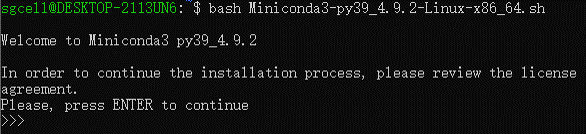
\includegraphics[width=0.55\linewidth]{./images/conda_init_conda} \end{center}

\begin{itemize}
\tightlist
\item
  Follow the prompts on the installer screens.
\end{itemize}

When you are asked \texttt{Do\ you\ wish\ the\ installer\ to\ initialize\ Miniconda3\ by\ running\ conda\ init}, we recommend ``yes''. When the initialization is done, it looks like,

\begin{center}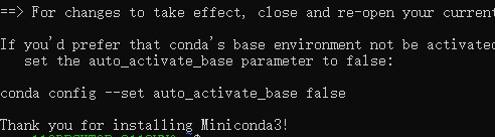
\includegraphics[width=0.45\linewidth]{./images/conda_init_conda2} \end{center}

\textbf{Step 5. Close and re-open Shell}

\begin{itemize}
\tightlist
\item
  Close and then re-open your Shell, to make the changes take effect.
\end{itemize}

The screen should have a new \texttt{(base)} prefix, which looks like,

\begin{center}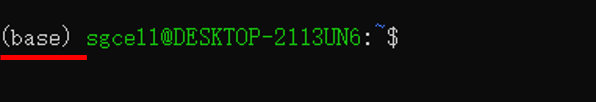
\includegraphics[width=0.4\linewidth]{./images/conda_reopen_shell} \end{center}

It means the Shell is now in the \texttt{base} environment of conda.

\textbf{Step 6. Test your installation}

\begin{itemize}
\tightlist
\item
  Type \texttt{conda\ list} in Shell.
\end{itemize}

A list of installed packages appears if it has been installed correctly.

\begin{center}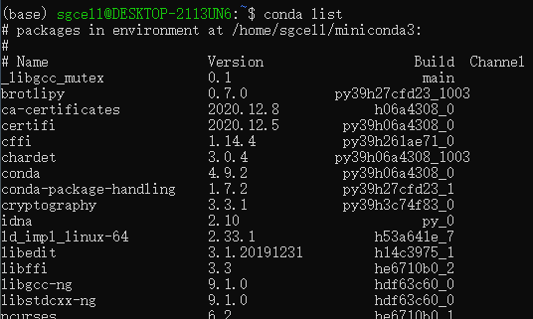
\includegraphics[width=0.5\linewidth]{./images/conda_test_conda} \end{center}

\hypertarget{conda_install_mac}{%
\subsection{Installation on macOS}\label{conda_install_mac}}

You could refer to the Section \protect\hyperlink{conda_install_linux}{Installation on Linux} as the processes of installing Miniconda on macOS and Linux are quite similar. We briefly list the steps here for your quick reference.

\textbf{Step 1. Open macOS Terminal}

\textbf{Step 2. Download Miniconda installer}

\begin{itemize}
\tightlist
\item
  Type in Terminal \texttt{wget\ https://repo.anaconda.com/miniconda/Miniconda3-py39\_4.9.2-MacOSX-x86\_64.sh}.
\end{itemize}

\textbf{Step 3. Verify your installer hashes (Optional)}

\begin{itemize}
\tightlist
\item
  Type \texttt{shasum\ -a\ 256\ Miniconda3-py39\_4.9.2-MacOSX-x86\_64.sh} in Terminal and check if the output hash is \texttt{b3bf77cbb81ee235ec6858146a2a84d20f8ecdeb614678030c39baacb5acbed1}.
\end{itemize}

\textbf{Step 4. Initialize Miniconda}

\begin{itemize}
\item
  Type in Terminal \texttt{bash\ Miniconda3-py39\_4.9.2-MacOSX-x86\_64.sh}.
\item
  Follow the prompts on the installer screens.
\end{itemize}

When you are asked \texttt{Do\ you\ wish\ the\ installer\ to\ initialize\ Miniconda3\ by\ running\ conda\ init}, we recommend ``yes''.

\textbf{Step 5. Close and re-open Terminal}

\textbf{Step 6. Test your installation}

\begin{itemize}
\tightlist
\item
  Type \texttt{conda\ list} in Terminal.
\end{itemize}

A list of installed packages appears if it has been installed correctly.

\hypertarget{other-prepare}{%
\section{other prepare}\label{other-prepare}}

\hypertarget{conda-configuration}{%
\subsection{Conda Configuration}\label{conda-configuration}}

To simplify the configuration of conda environment, we have pre-compiled a conda environment, named \texttt{sgcell}, containing all required softwares for this workshop. The corresponding metafile \texttt{sgcell.yml} of this environment was exported, based on which we can easily re-build the pre-compiled environment.

Assuming you have installed conda and activated any environment in the Shell / Terminal (if not, please install conda based on Section \protect\hyperlink{conda_install}{Install Conda Environment} first). Then,

\begin{itemize}
\item
  Open Linux Shell / macOS Terminal / WSL Shell
\item
  Add conda channels,
\end{itemize}

\begin{verbatim}
conda config --add channels bioconda
conda config --add channels conda-forge
\end{verbatim}

\begin{itemize}
\tightlist
\item
  Re-build the pre-compiled environment,
\end{itemize}

\begin{verbatim}
conda env create -f sgcell.yml
\end{verbatim}

\begin{itemize}
\tightlist
\item
  Activate the new environment \texttt{sgcell},
\end{itemize}

\begin{verbatim}
conda activate sgcell
\end{verbatim}

\begin{itemize}
\tightlist
\item
  Verify if the new environment was installed correctly,
\end{itemize}

\begin{verbatim}
conda env list
\end{verbatim}

The \texttt{sgcell} sould appear in the listed environments.

\hypertarget{example-of-r-markdown}{%
\subsection{Example of R Markdown}\label{example-of-r-markdown}}

You can label chapter and section titles using \texttt{\{\#label\}} after them, e.g., we can reference Chapter \ref{env-pre}. If you do not manually label them, there will be automatic labels anyway, e.g., Chapter @ref(RNA velocity).

Figures and tables with captions will be placed in \texttt{figure} and \texttt{table} environments, respectively.

\begin{Shaded}
\begin{Highlighting}[]
\KeywordTok{par}\NormalTok{(}\DataTypeTok{mar =} \KeywordTok{c}\NormalTok{(}\DecValTok{4}\NormalTok{, }\DecValTok{4}\NormalTok{, }\FloatTok{.1}\NormalTok{, }\FloatTok{.1}\NormalTok{))}
\KeywordTok{plot}\NormalTok{(pressure, }\DataTypeTok{type =} \StringTok{\textquotesingle{}b\textquotesingle{}}\NormalTok{, }\DataTypeTok{pch =} \DecValTok{19}\NormalTok{)}
\end{Highlighting}
\end{Shaded}

\begin{figure}

{\centering 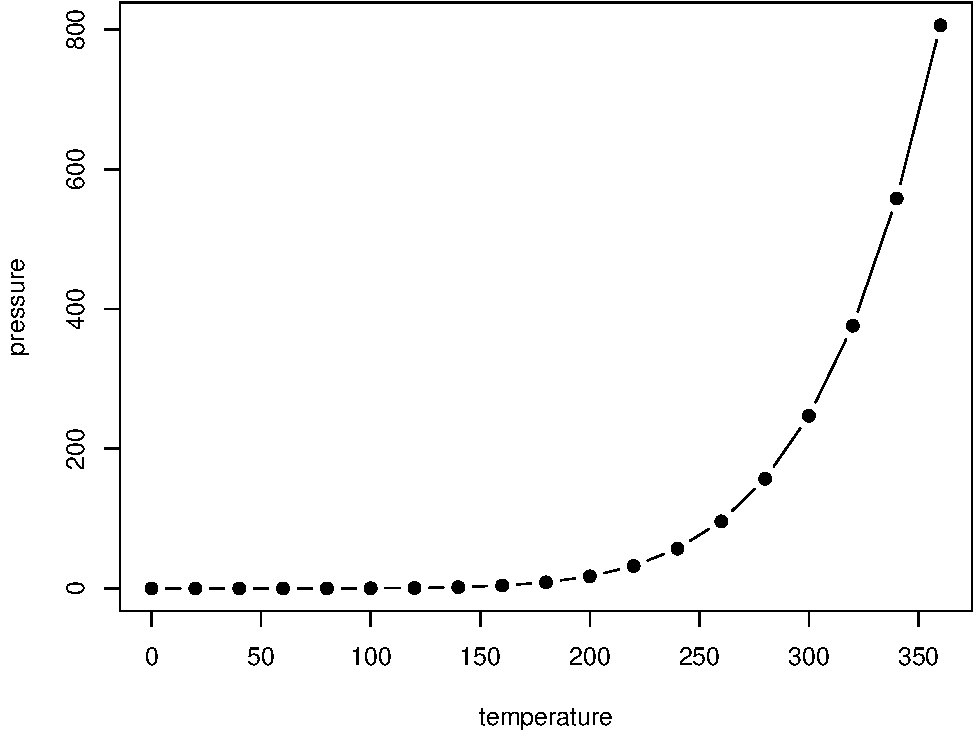
\includegraphics[width=0.8\linewidth]{SingleCell-Workshop_files/figure-latex/nice-fig-1} 

}

\caption{Here is a nice figure!}\label{fig:nice-fig}
\end{figure}

Reference a figure by its code chunk label with the \texttt{fig:} prefix, e.g., see Figure \ref{fig:nice-fig}. Similarly, you can reference tables generated from \texttt{knitr::kable()}, e.g., see Table \ref{tab:nice-tab}.

\begin{Shaded}
\begin{Highlighting}[]
\NormalTok{knitr}\OperatorTok{::}\KeywordTok{kable}\NormalTok{(}
  \KeywordTok{head}\NormalTok{(iris, }\DecValTok{20}\NormalTok{), }\DataTypeTok{caption =} \StringTok{\textquotesingle{}Here is a nice table!\textquotesingle{}}\NormalTok{,}
  \DataTypeTok{booktabs =} \OtherTok{TRUE}
\NormalTok{)}
\end{Highlighting}
\end{Shaded}

\begin{table}

\caption{\label{tab:nice-tab}Here is a nice table!}
\centering
\begin{tabular}[t]{rrrrl}
\toprule
Sepal.Length & Sepal.Width & Petal.Length & Petal.Width & Species\\
\midrule
5.1 & 3.5 & 1.4 & 0.2 & setosa\\
4.9 & 3.0 & 1.4 & 0.2 & setosa\\
4.7 & 3.2 & 1.3 & 0.2 & setosa\\
4.6 & 3.1 & 1.5 & 0.2 & setosa\\
5.0 & 3.6 & 1.4 & 0.2 & setosa\\
\addlinespace
5.4 & 3.9 & 1.7 & 0.4 & setosa\\
4.6 & 3.4 & 1.4 & 0.3 & setosa\\
5.0 & 3.4 & 1.5 & 0.2 & setosa\\
4.4 & 2.9 & 1.4 & 0.2 & setosa\\
4.9 & 3.1 & 1.5 & 0.1 & setosa\\
\addlinespace
5.4 & 3.7 & 1.5 & 0.2 & setosa\\
4.8 & 3.4 & 1.6 & 0.2 & setosa\\
4.8 & 3.0 & 1.4 & 0.1 & setosa\\
4.3 & 3.0 & 1.1 & 0.1 & setosa\\
5.8 & 4.0 & 1.2 & 0.2 & setosa\\
\addlinespace
5.7 & 4.4 & 1.5 & 0.4 & setosa\\
5.4 & 3.9 & 1.3 & 0.4 & setosa\\
5.1 & 3.5 & 1.4 & 0.3 & setosa\\
5.7 & 3.8 & 1.7 & 0.3 & setosa\\
5.1 & 3.8 & 1.5 & 0.3 & setosa\\
\bottomrule
\end{tabular}
\end{table}

You can write citations, too. For example, we are using the \textbf{bookdown} package \citep{R-bookdown} in this sample book, which was built on top of R Markdown and \textbf{knitr} \citep{xie2015}.

This is a \emph{sample} book written in \textbf{Markdown}. You can use anything that Pandoc's Markdown supports, e.g., a math equation \(a^2 + b^2 = c^2\).

The \textbf{bookdown} package can be installed from CRAN or Github:

\begin{Shaded}
\begin{Highlighting}[]
\KeywordTok{install.packages}\NormalTok{(}\StringTok{"bookdown"}\NormalTok{)}
\CommentTok{\# or the development version}
\CommentTok{\# devtools::install\_github("rstudio/bookdown")}
\end{Highlighting}
\end{Shaded}

Remember each Rmd file contains one and only one chapter, and a chapter is defined by the first-level heading \texttt{\#}.

To compile this example to PDF, you need XeLaTeX. You are recommended to install TinyTeX (which includes XeLaTeX): \url{https://yihui.org/tinytex/}.

\hypertarget{pseudo-time-and-trajectory-analysis}{%
\chapter{Pseudo-time and trajectory analysis}\label{pseudo-time-and-trajectory-analysis}}

Here is a review of existing methods.

\hypertarget{rna-velocity}{%
\chapter{RNA velocity}\label{rna-velocity}}

We describe our methods in this chapter.

\hypertarget{copy-number-variation-estimation-from-scrna-seq}{%
\chapter{Copy number variation estimation from scRNA-seq}\label{copy-number-variation-estimation-from-scrna-seq}}

Rongting Huang

2021-06-29

\hypertarget{method-infercnv}{%
\section{Method: inferCNV}\label{method-infercnv}}

\href{https://github.com/broadinstitute/inferCNV/wiki}{InferCNV: Inferring copy number alterations from tumor single cell RNA-Seq data}

\hypertarget{install-infercnv}{%
\subsection{install inferCNV}\label{install-infercnv}}

\textbf{Software Requirements}

\begin{itemize}
\tightlist
\item
  \href{https://mcmc-jags.sourceforge.io/}{JAGS}
\item
  R (\textgreater3.6)
\end{itemize}

In order to run infercnv, JAGS (Just Another Gibbs Sampler) must be installed.

Download JAGS from \url{https://sourceforge.net/projects/mcmc-jags/files/JAGS/4.x/} and install JAGS in your environment (windows/MAC).

If you use inferCNV on server, install JAGS via \texttt{conda\ install} in your conda environment is recommended.

\begin{verbatim}
conda install -c conda-forge jags
\end{verbatim}

More details refer to \href{https://github.com/broadinstitute/inferCNV/wiki}{inferCNV wiki page}

\textbf{Five options for installing inferCNV}

Option A: Install infercnv from BioConductor (preferred)

\begin{verbatim}
if (!requireNamespace("BiocManager", quietly = TRUE))
     install.packages("BiocManager")
BiocManager::install("infercnv")
\end{verbatim}

For more other options, refer to \href{https://github.com/broadinstitute/inferCNV/wiki/Installing-infercnv}{Five options for installing inferCNV}

\textbf{Data requirements}

\begin{itemize}
\tightlist
\item
  a raw counts matrix of single-cell RNA-Seq expression
\item
  an annotations file which indicates which cells are tumor vs.~normal.
\item
  a gene/chromosome positions file
\end{itemize}

\href{https://github.com/broadinstitute/inferCNV/wiki/File-Definitions}{File-Definitions}

\hypertarget{getting-started}{%
\subsection{getting started}\label{getting-started}}

If you have installed infercnv from BioConductor, you can run the example data with:

\begin{verbatim}
library(infercnv)

infercnv_obj = CreateInfercnvObject(raw_counts_matrix=system.file("extdata", "oligodendroglioma_expression_downsampled.counts.matrix.gz", package = "infercnv"),
                                    annotations_file=system.file("extdata", "oligodendroglioma_annotations_downsampled.txt", package = "infercnv"),
                                    delim="\t",
                                    gene_order_file=system.file("extdata", "gencode_downsampled.EXAMPLE_ONLY_DONT_REUSE.txt", package = "infercnv"),
                                    ref_group_names=c("Microglia/Macrophage","Oligodendrocytes (non-malignant)")) 

infercnv_obj = infercnv::run(infercnv_obj,
                             cutoff=1, # cutoff=1 works well for Smart-seq2, and cutoff=0.1 works well for 10x Genomics
                             out_dir=tempfile(), 
                             cluster_by_groups=TRUE, 
                             denoise=TRUE,
                             HMM=TRUE)
\end{verbatim}

If you can run the getting started part with demo data provided by inferCNV, then it is installed successfully.

\textbf{Demo Example Figure}

\begin{figure}
\centering
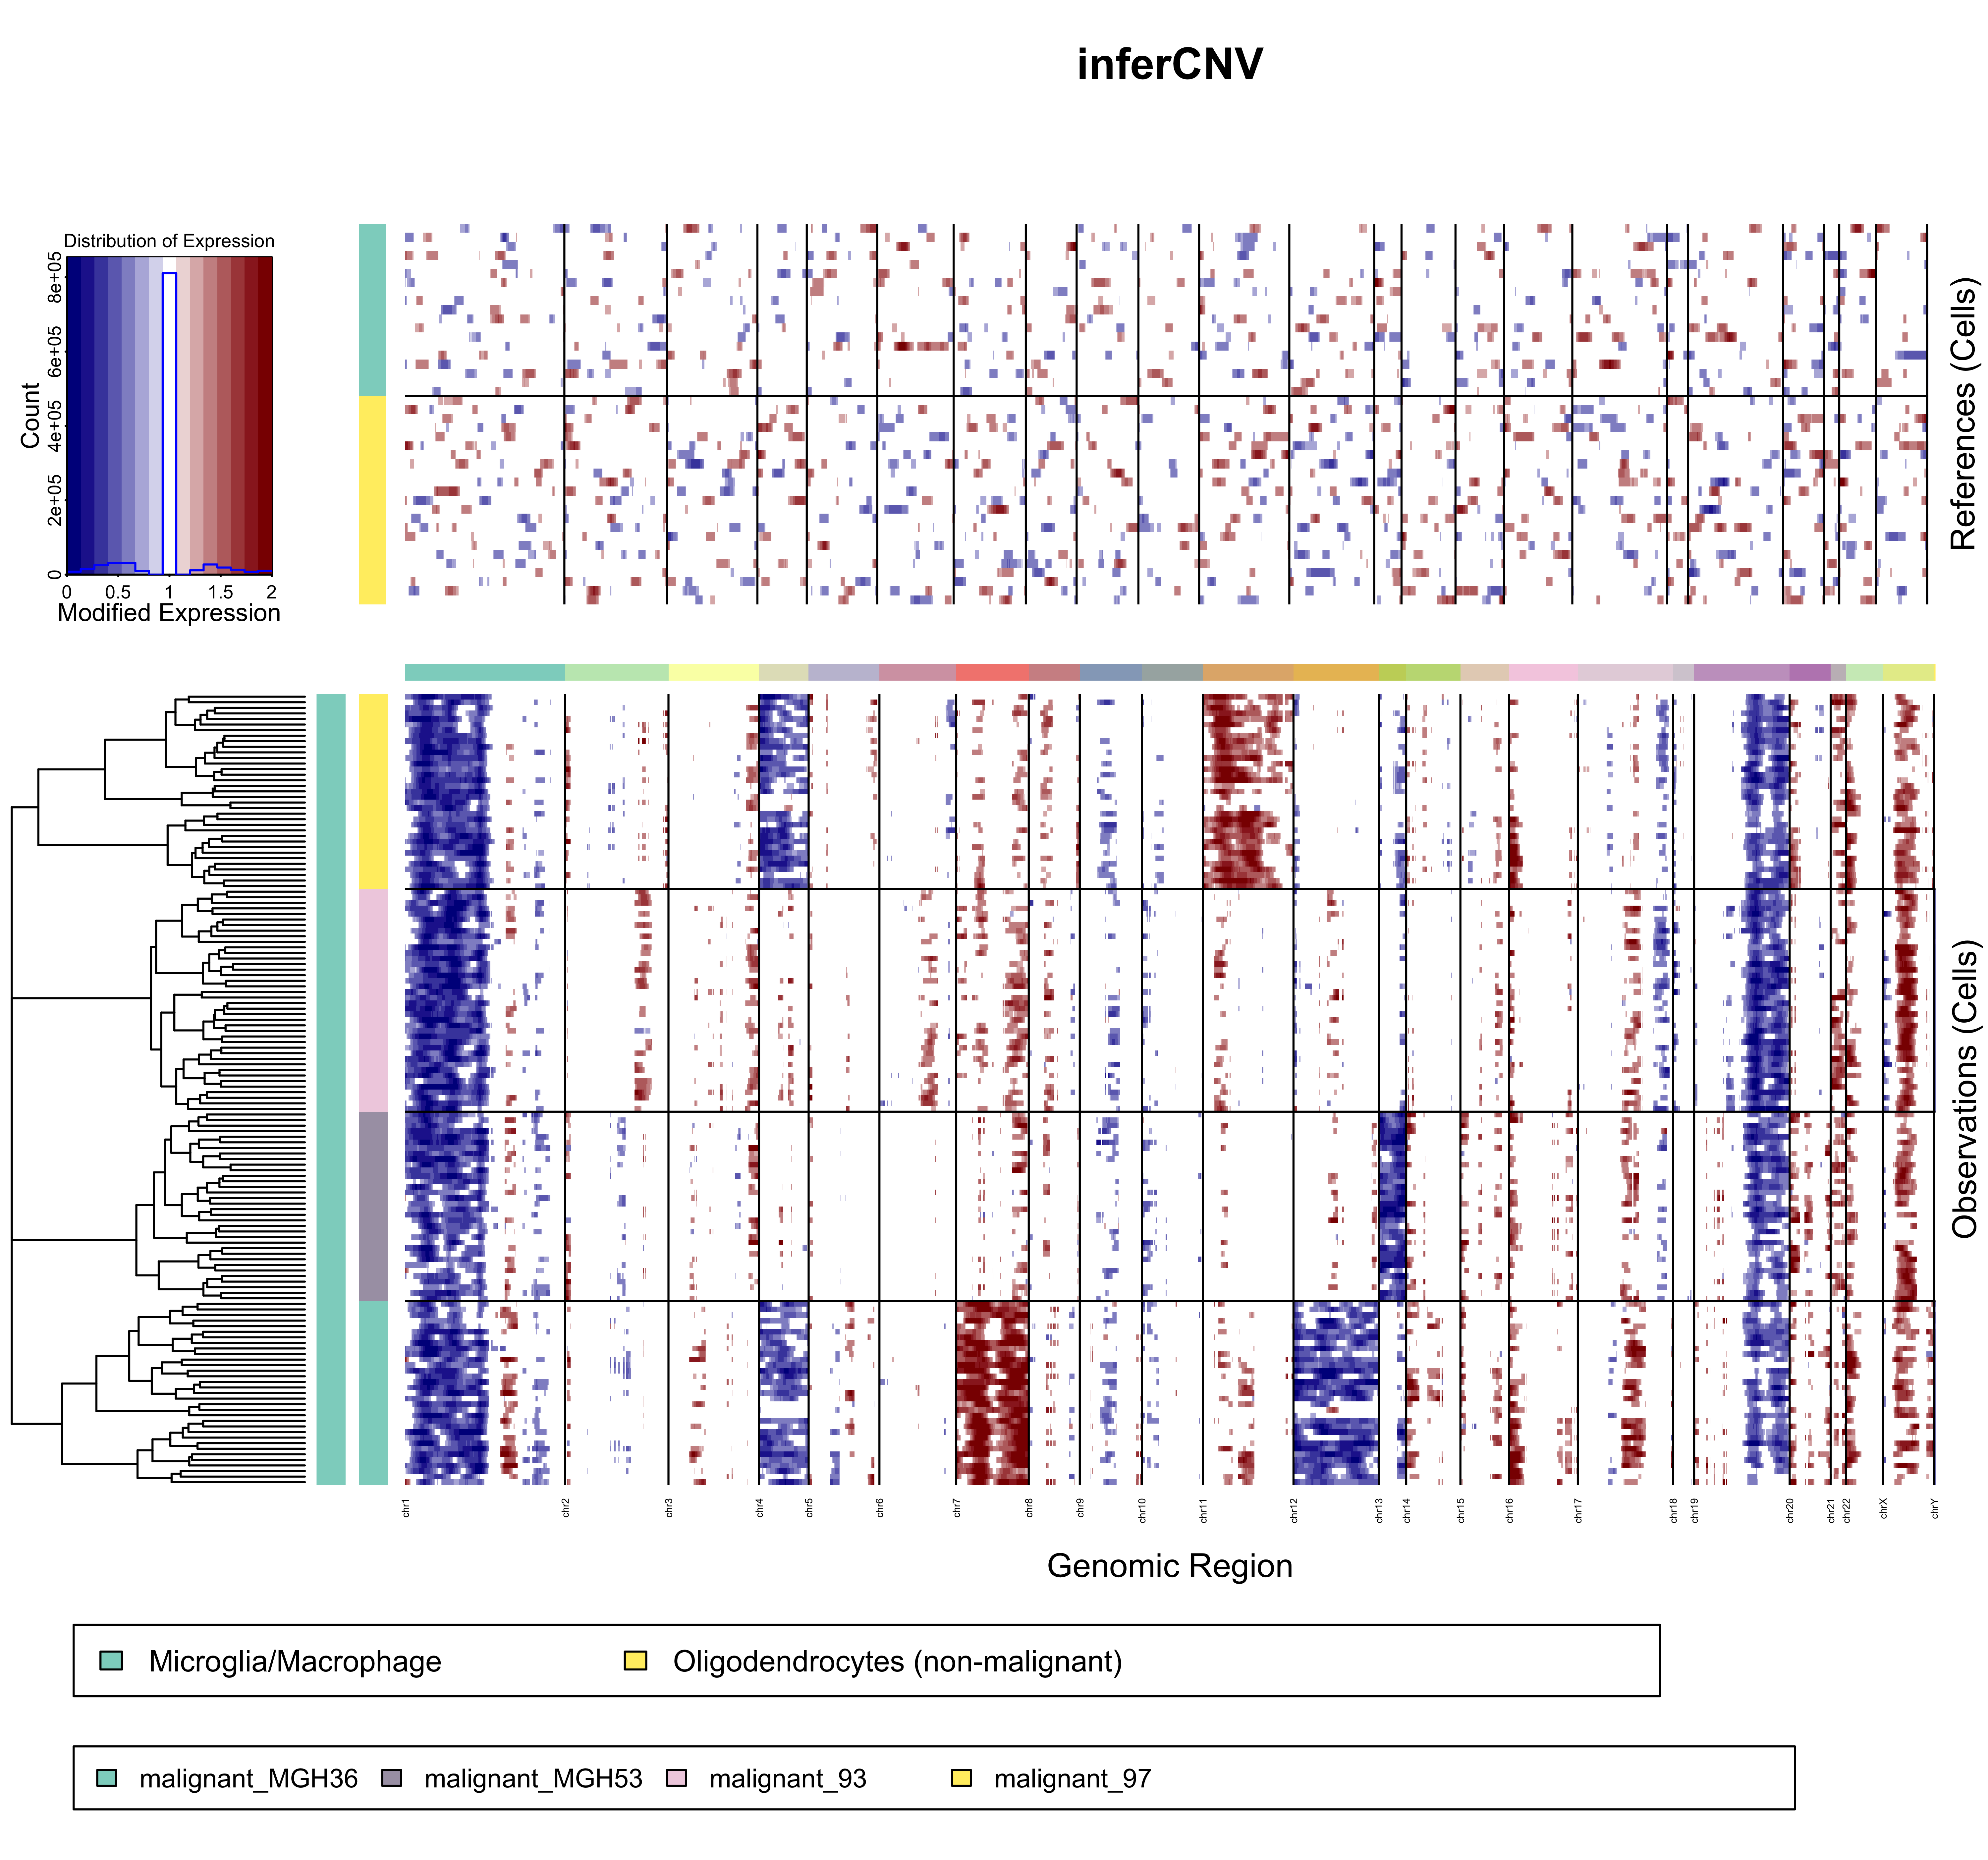
\includegraphics{CNV_analysis_file/figs/demo-infercnv.png}
\caption{Demo Example Figure}
\end{figure}

\hypertarget{application-on-tnbc1}{%
\section{Application on TNBC1}\label{application-on-tnbc1}}

\hypertarget{data-description}{%
\subsection{data description}\label{data-description}}

TNBC1 is a triple negative breast cancer tumor sample of high tumor purity (72.6\%) with 796 single tumor cells and 301 normal cells. The dataset is available on NCBI GEO under the accession number GSM4476486.

\begin{longtable}[]{@{}llll@{}}
\caption{Details of TNBC1 dataset (from published articles, copyKAT).}\tabularnewline
\toprule
\begin{minipage}[b]{0.25\columnwidth}\raggedright
TNBC1\strut
\end{minipage} & \begin{minipage}[b]{0.16\columnwidth}\raggedright
Number of clones\strut
\end{minipage} & \begin{minipage}[b]{0.19\columnwidth}\raggedright
Number of tumor clones\strut
\end{minipage} & \begin{minipage}[b]{0.29\columnwidth}\raggedright
Tumor clone-specific copy gain\strut
\end{minipage}\tabularnewline
\midrule
\endfirsthead
\toprule
\begin{minipage}[b]{0.25\columnwidth}\raggedright
TNBC1\strut
\end{minipage} & \begin{minipage}[b]{0.16\columnwidth}\raggedright
Number of clones\strut
\end{minipage} & \begin{minipage}[b]{0.19\columnwidth}\raggedright
Number of tumor clones\strut
\end{minipage} & \begin{minipage}[b]{0.29\columnwidth}\raggedright
Tumor clone-specific copy gain\strut
\end{minipage}\tabularnewline
\midrule
\endhead
\begin{minipage}[t]{0.25\columnwidth}\raggedright
Triple negative breast cancer\strut
\end{minipage} & \begin{minipage}[t]{0.16\columnwidth}\raggedright
\begin{verbatim}
    3
\end{verbatim}
\strut
\end{minipage} & \begin{minipage}[t]{0.19\columnwidth}\raggedright
\begin{verbatim}
        2
\end{verbatim}
\strut
\end{minipage} & \begin{minipage}[t]{0.29\columnwidth}\raggedright
\begin{itemize}
\tightlist
\item
  C1: 4p, 7q, 9, 17q
\item
  C2: 3p, 6q, 7p, 11q, X
\end{itemize}\strut
\end{minipage}\tabularnewline
\bottomrule
\end{longtable}

\begin{itemize}
\tightlist
\item
  Expression
\end{itemize}

\begin{longtable}[]{@{}lll@{}}
\caption{Subclusters of TNBC1 dataset (from gene expression analysis-Seurat).}\tabularnewline
\toprule
Clone A & Clone B & Normal\tabularnewline
\midrule
\endfirsthead
\toprule
Clone A & Clone B & Normal\tabularnewline
\midrule
\endhead
488 & 307 & 302\tabularnewline
\bottomrule
\end{longtable}

Notes: 488,307, 247, 55

\begin{figure}
\centering
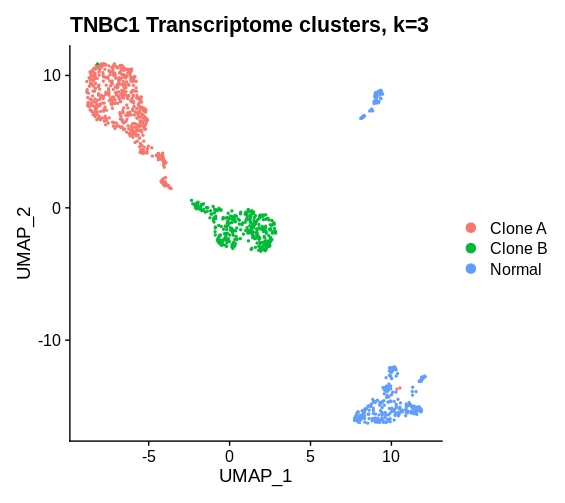
\includegraphics{CNV_analysis_file/figs/tnbc1-exp/tnbc1-umap-3clusters.jpeg}
\caption{umap}
\end{figure}

\begin{itemize}
\tightlist
\item
  B Allele Frenquency (BAF)
\end{itemize}

\begin{figure}
\centering
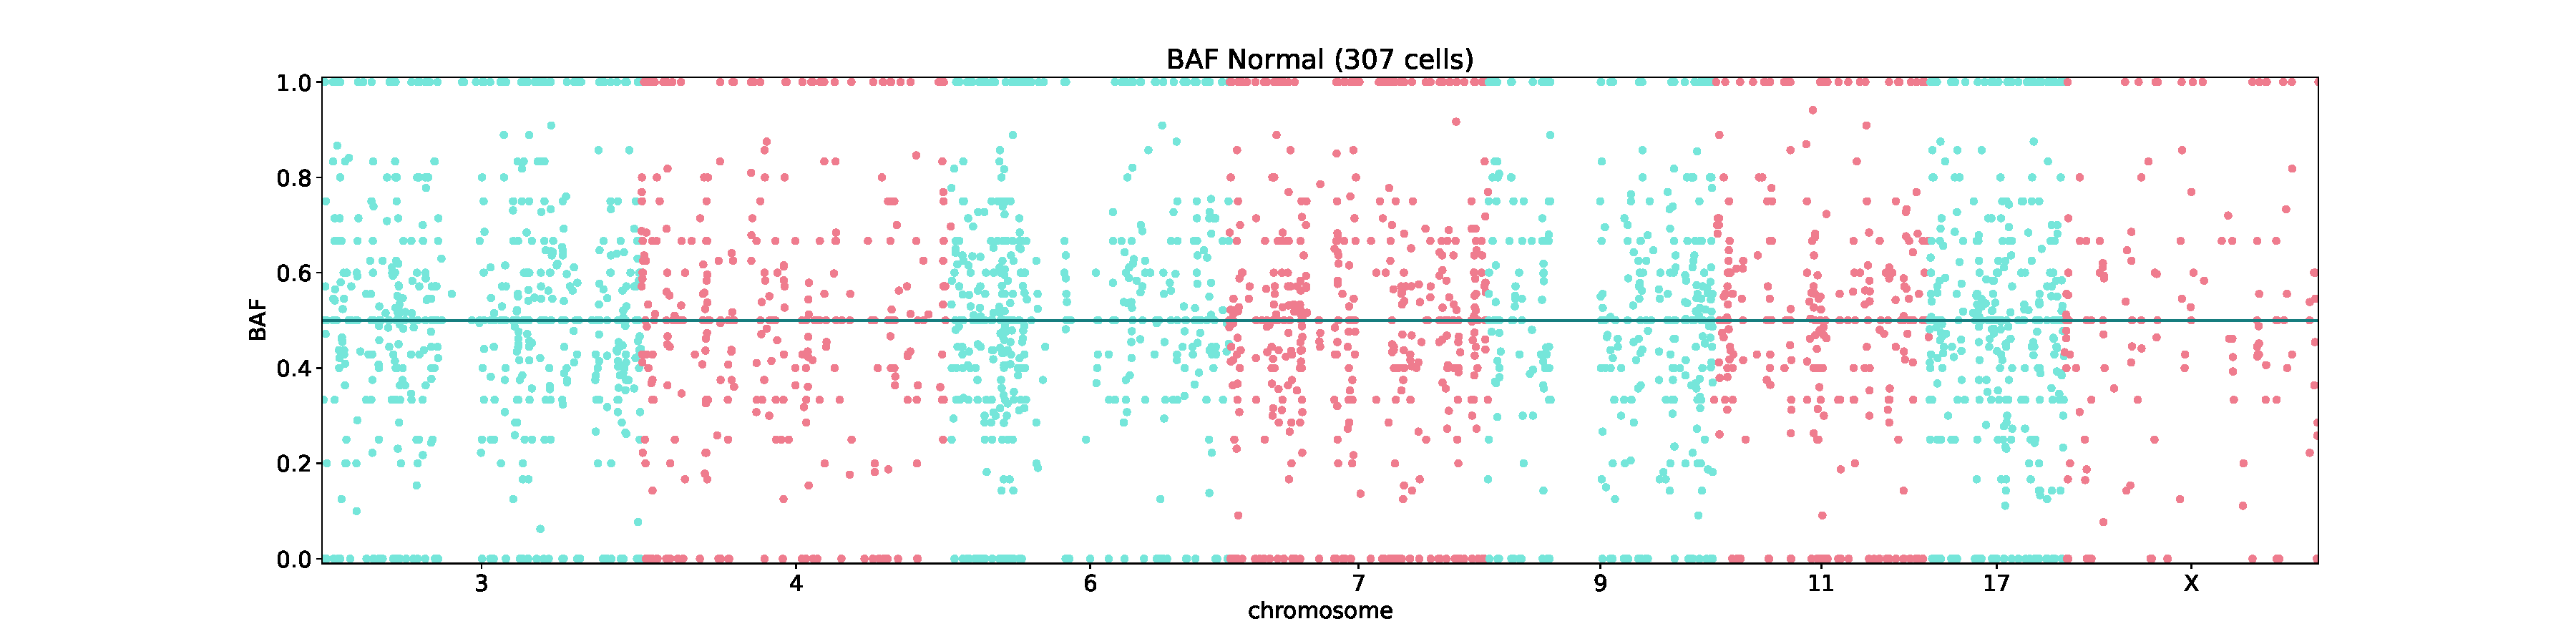
\includegraphics[width=1.2\textwidth,height=\textheight]{./CNV_analysis_file/figs/tnbc1-baf/0sub_chr.pdf}
\caption{baf1}
\end{figure}

\begin{figure}
\centering
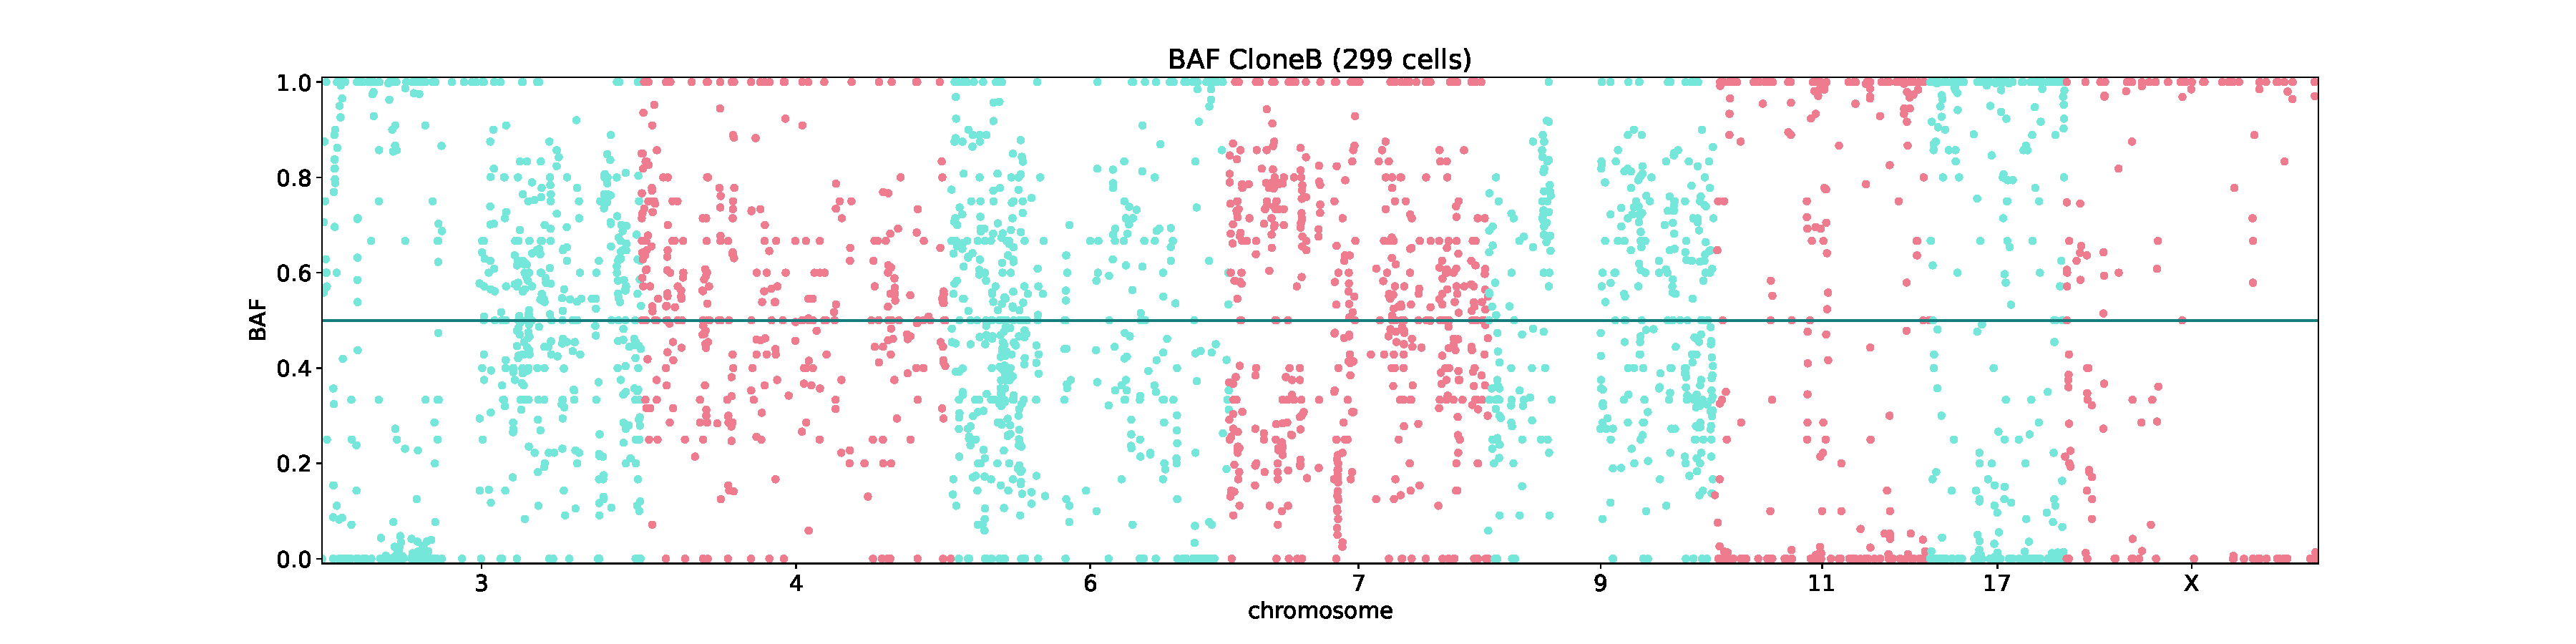
\includegraphics[width=1.2\textwidth,height=\textheight]{./CNV_analysis_file/figs/tnbc1-baf/1sub_chr.pdf}
\caption{baf2}
\end{figure}

\begin{figure}
\centering
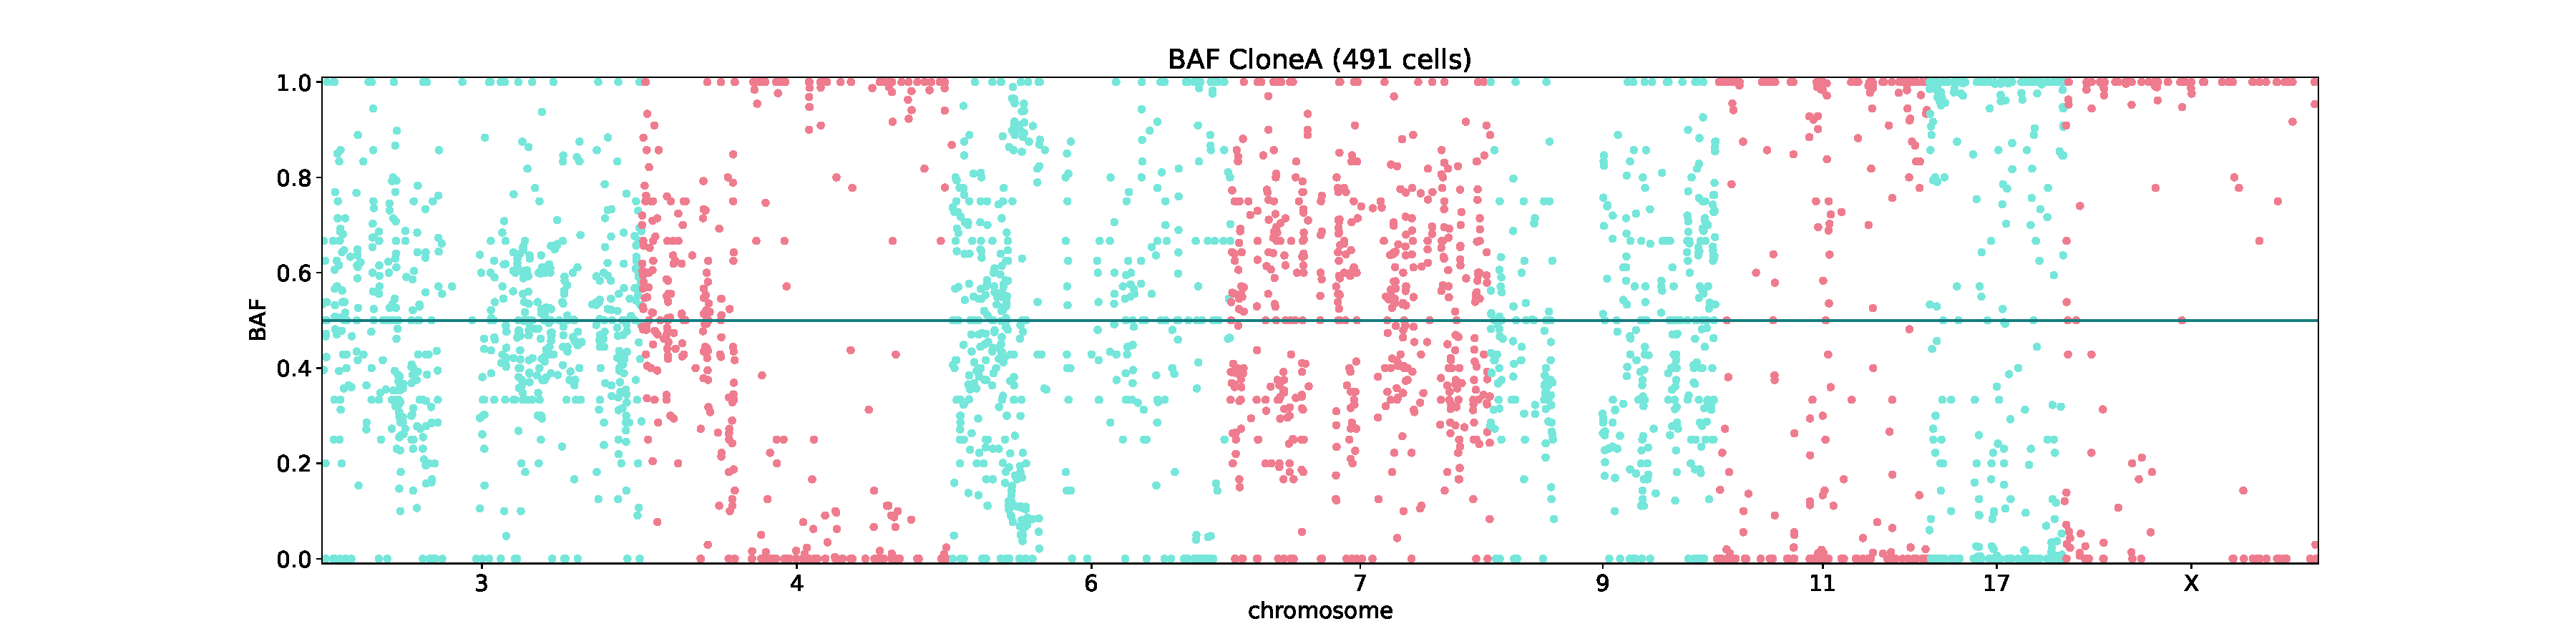
\includegraphics[width=1.2\textwidth,height=\textheight]{./CNV_analysis_file/figs/tnbc1-baf/2sub_chr.pdf}
\caption{baf3}
\end{figure}

\begin{itemize}
\tightlist
\item
  BAF V.S. Expression
\end{itemize}

\begin{figure}
\centering
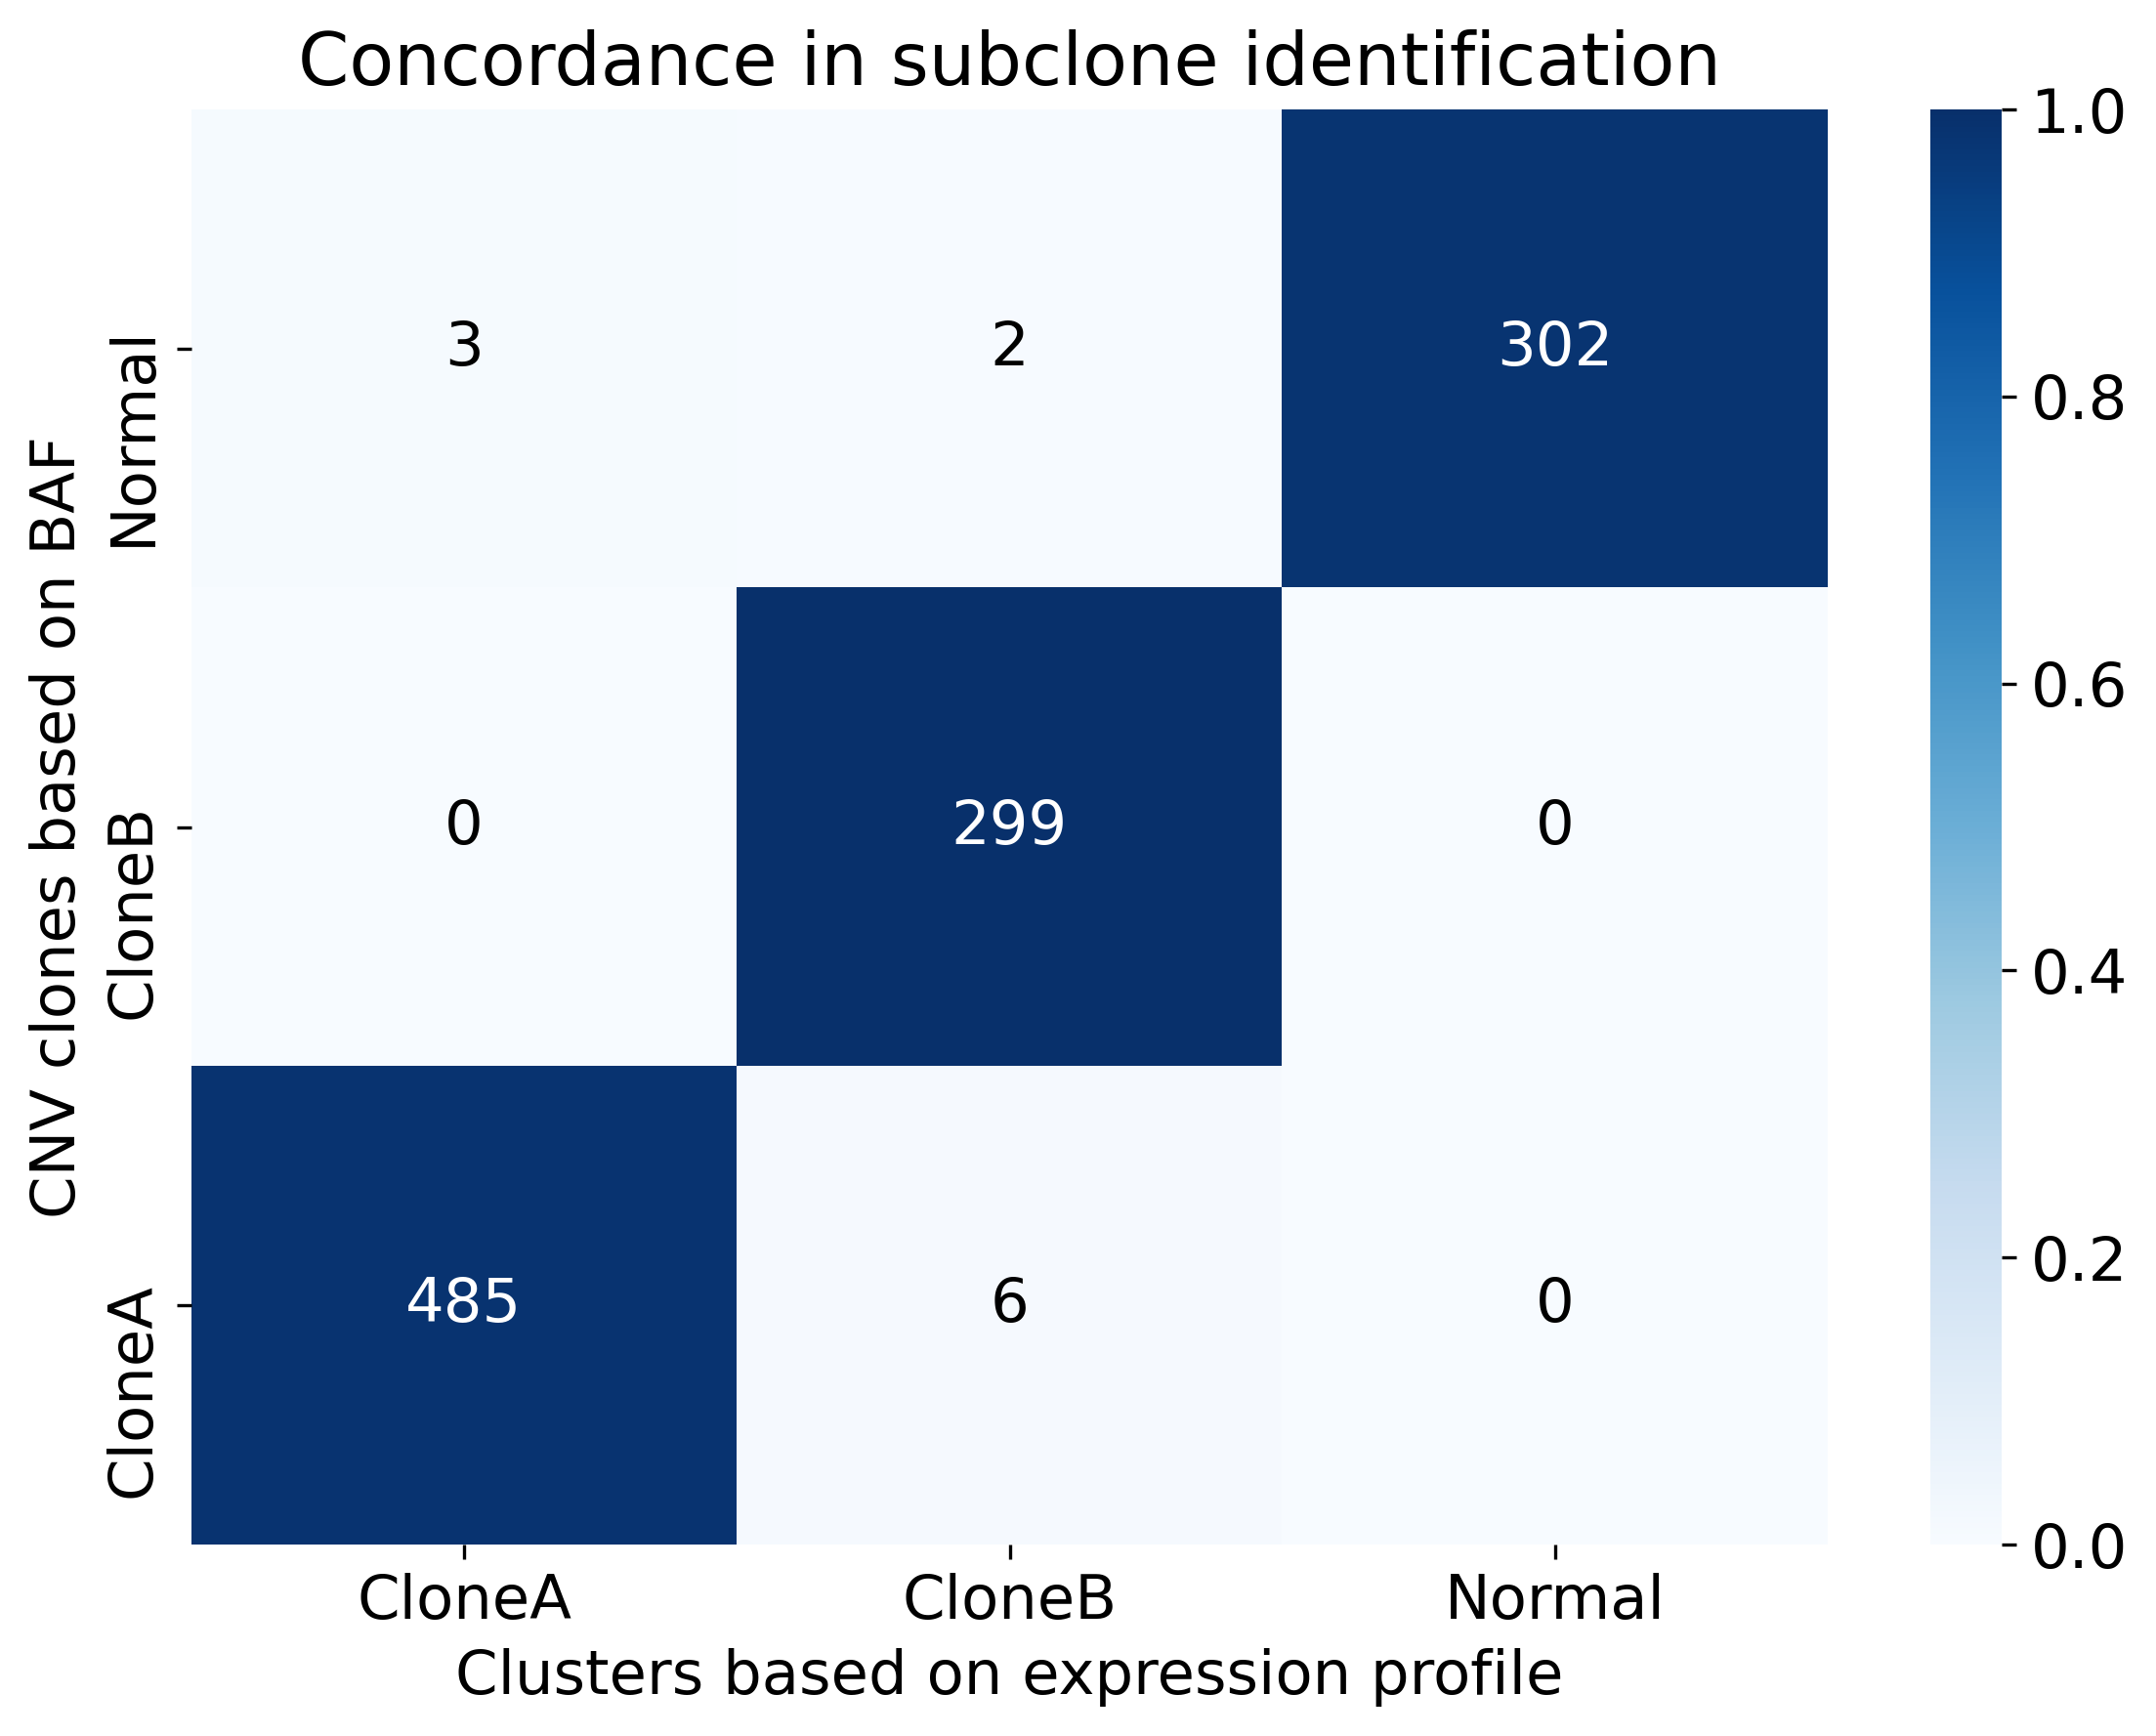
\includegraphics{CNV_analysis_file/figs/BAFvsExpression.png}
\caption{confusion heatmap}
\end{figure}

\hypertarget{run-infercnv}{%
\subsection{run inferCNV}\label{run-infercnv}}

\href{https://sourceforge.net/projects/sgcellworkshop/files/CNV_analysis/CNV_analysis_data.zip/download}{data\_download}

\href{https://github.com/Rongtingting/SingleCell-Workshop-2021/blob/master/CNV_analysis_file/demo1_inferCNV_TNBC1.log}{demo1\_log\_file}

\href{https://github.com/Rongtingting/SingleCell-Workshop-2021/blob/master/CNV_analysis_file/demo2_inferCNV_TNBC1.log}{demo2\_log\_file}

\href{https://github.com/Rongtingting/SingleCell-Workshop-2021/blob/master/CNV_analysis_file/demo2_outputfiles.lst}{output\_files}

\begin{Shaded}
\begin{Highlighting}[]
\CommentTok{\# library(infercnv)}
\CommentTok{\# library(utils)}
\CommentTok{\# library (BiocGenerics)}

\CommentTok{\#\# DEMO1}
\CommentTok{\# }
\CommentTok{\# tnbc \textless{}{-} read.delim("C://Users/Rongting/Documents/GitHub\_repos/combinedTNBC1.txt")}
\CommentTok{\# anno \textless{}{-} tnbc[2,]}
\CommentTok{\# anno \textless{}{-} t(anno)}
\CommentTok{\# anno \textless{}{-} as.data.frame(anno)}
\CommentTok{\# }
\CommentTok{\# gex \textless{}{-} tnbc[{-}c(1:2),]}
\CommentTok{\# gex \textless{}{-} type.convert(gex)}
\CommentTok{\# }
\CommentTok{\# gene\_file \textless{}{-} "C://Users/Rongting/Documents/GitHub\_repos/gene\_note\_noheader\_unique.txt"}

\CommentTok{\# }
\CommentTok{\# infercnv\_obj = CreateInfercnvObject(raw\_counts\_matrix=gex,}
\CommentTok{\#                                     annotations\_file=anno,}
\CommentTok{\#                                     delim=\textquotesingle{}\textbackslash{}t\textquotesingle{},}
\CommentTok{\#                                     gene\_order\_file=gene\_file,}
\CommentTok{\#                                     ref\_group\_names= "N")}

\CommentTok{\# output = "C://Users/Rongting/Documents/GitHub\_repos/tnbc1\_demo"}

\CommentTok{\# infercnv\_obj = infercnv::run(infercnv\_obj,}
\CommentTok{\#                              cutoff=0.1,  }
\CommentTok{\#                              out\_dir= output , }
\CommentTok{\#                              cluster\_by\_groups=T,   }
\CommentTok{\#                              denoise=T,}
\CommentTok{\#                              HMM=T)}

\CommentTok{\#\# DEMO2}

\CommentTok{\# gene\_file \textless{}{-} "C://Users/Rongting/Documents/GitHub\_repos/gene\_note\_noheader\_unique.txt"}
\CommentTok{\# }
\CommentTok{\# anno\_file \textless{}{-} \textquotesingle{}C://Users/Rongting/Documents/GitHub\_repos/tnbc{-}3cluster{-}id.txt\textquotesingle{}}
\CommentTok{\# }
\CommentTok{\# infercnv\_obj2 = CreateInfercnvObject(raw\_counts\_matrix=gex,}
\CommentTok{\#                                     annotations\_file=anno\_file,}
\CommentTok{\#                                     delim=\textquotesingle{}\textbackslash{}t\textquotesingle{},}
\CommentTok{\#                                     gene\_order\_file=gene\_file,}
\CommentTok{\#                                     ref\_group\_names= "Normal")}
\CommentTok{\# }
\CommentTok{\# output = "C://Users/Rongting/Documents/GitHub\_repos/tnbc1\_demo2"}
\CommentTok{\# }
\CommentTok{\# infercnv\_obj2 = infercnv::run(infercnv\_obj2,}
\CommentTok{\#                              cutoff=0.1,}
\CommentTok{\#                              out\_dir= output,}
\CommentTok{\#                              cluster\_by\_groups=T,}
\CommentTok{\#                              denoise=T,}
\CommentTok{\#                              HMM=T)}
\end{Highlighting}
\end{Shaded}

\begin{verbatim}
#################
##Notes
#################

## load the package
library(Seurat)
library(infercnv)

## prepare the data (cellranger output)

### load count matrix (example)
matrix_path <- "../cellranger/xxxx/count_xxxxx/outs/filtered_gene_bc_matrices/GRCh38/"


### read count matrix
gex_mtx <- Seurat::Read10X(data.dir = matrix_path)

### run inferCNV with loop
celltype = c('CloneA', 'CloneB', 'Normal')

for (i in celltype){
  infercnv_obj1 = CreateInfercnvObject(raw_counts_matrix=gex_mtx,
                                       annotations_file=anno_file,
                                       delim='\t',
                                       gene_order_file=gene_file,
                                       ref_group_names=c(i))
  
  output <- paste0('/groups/cgsd/rthuang/processed_data/inferCNV/xxxx/','xxxx_', i)
  
  infercnv_obj1 = infercnv::run(infercnv_obj1,
                                cutoff=0.1,  
                                out_dir= output , 
                                cluster_by_groups=T,   
                                denoise=T,
                                HMM=T)
}
\end{verbatim}

\hypertarget{infercnv-result}{%
\subsection{inferCNV result}\label{infercnv-result}}

\begin{itemize}
\tightlist
\item
  demo1
\end{itemize}

\begin{figure}
\centering
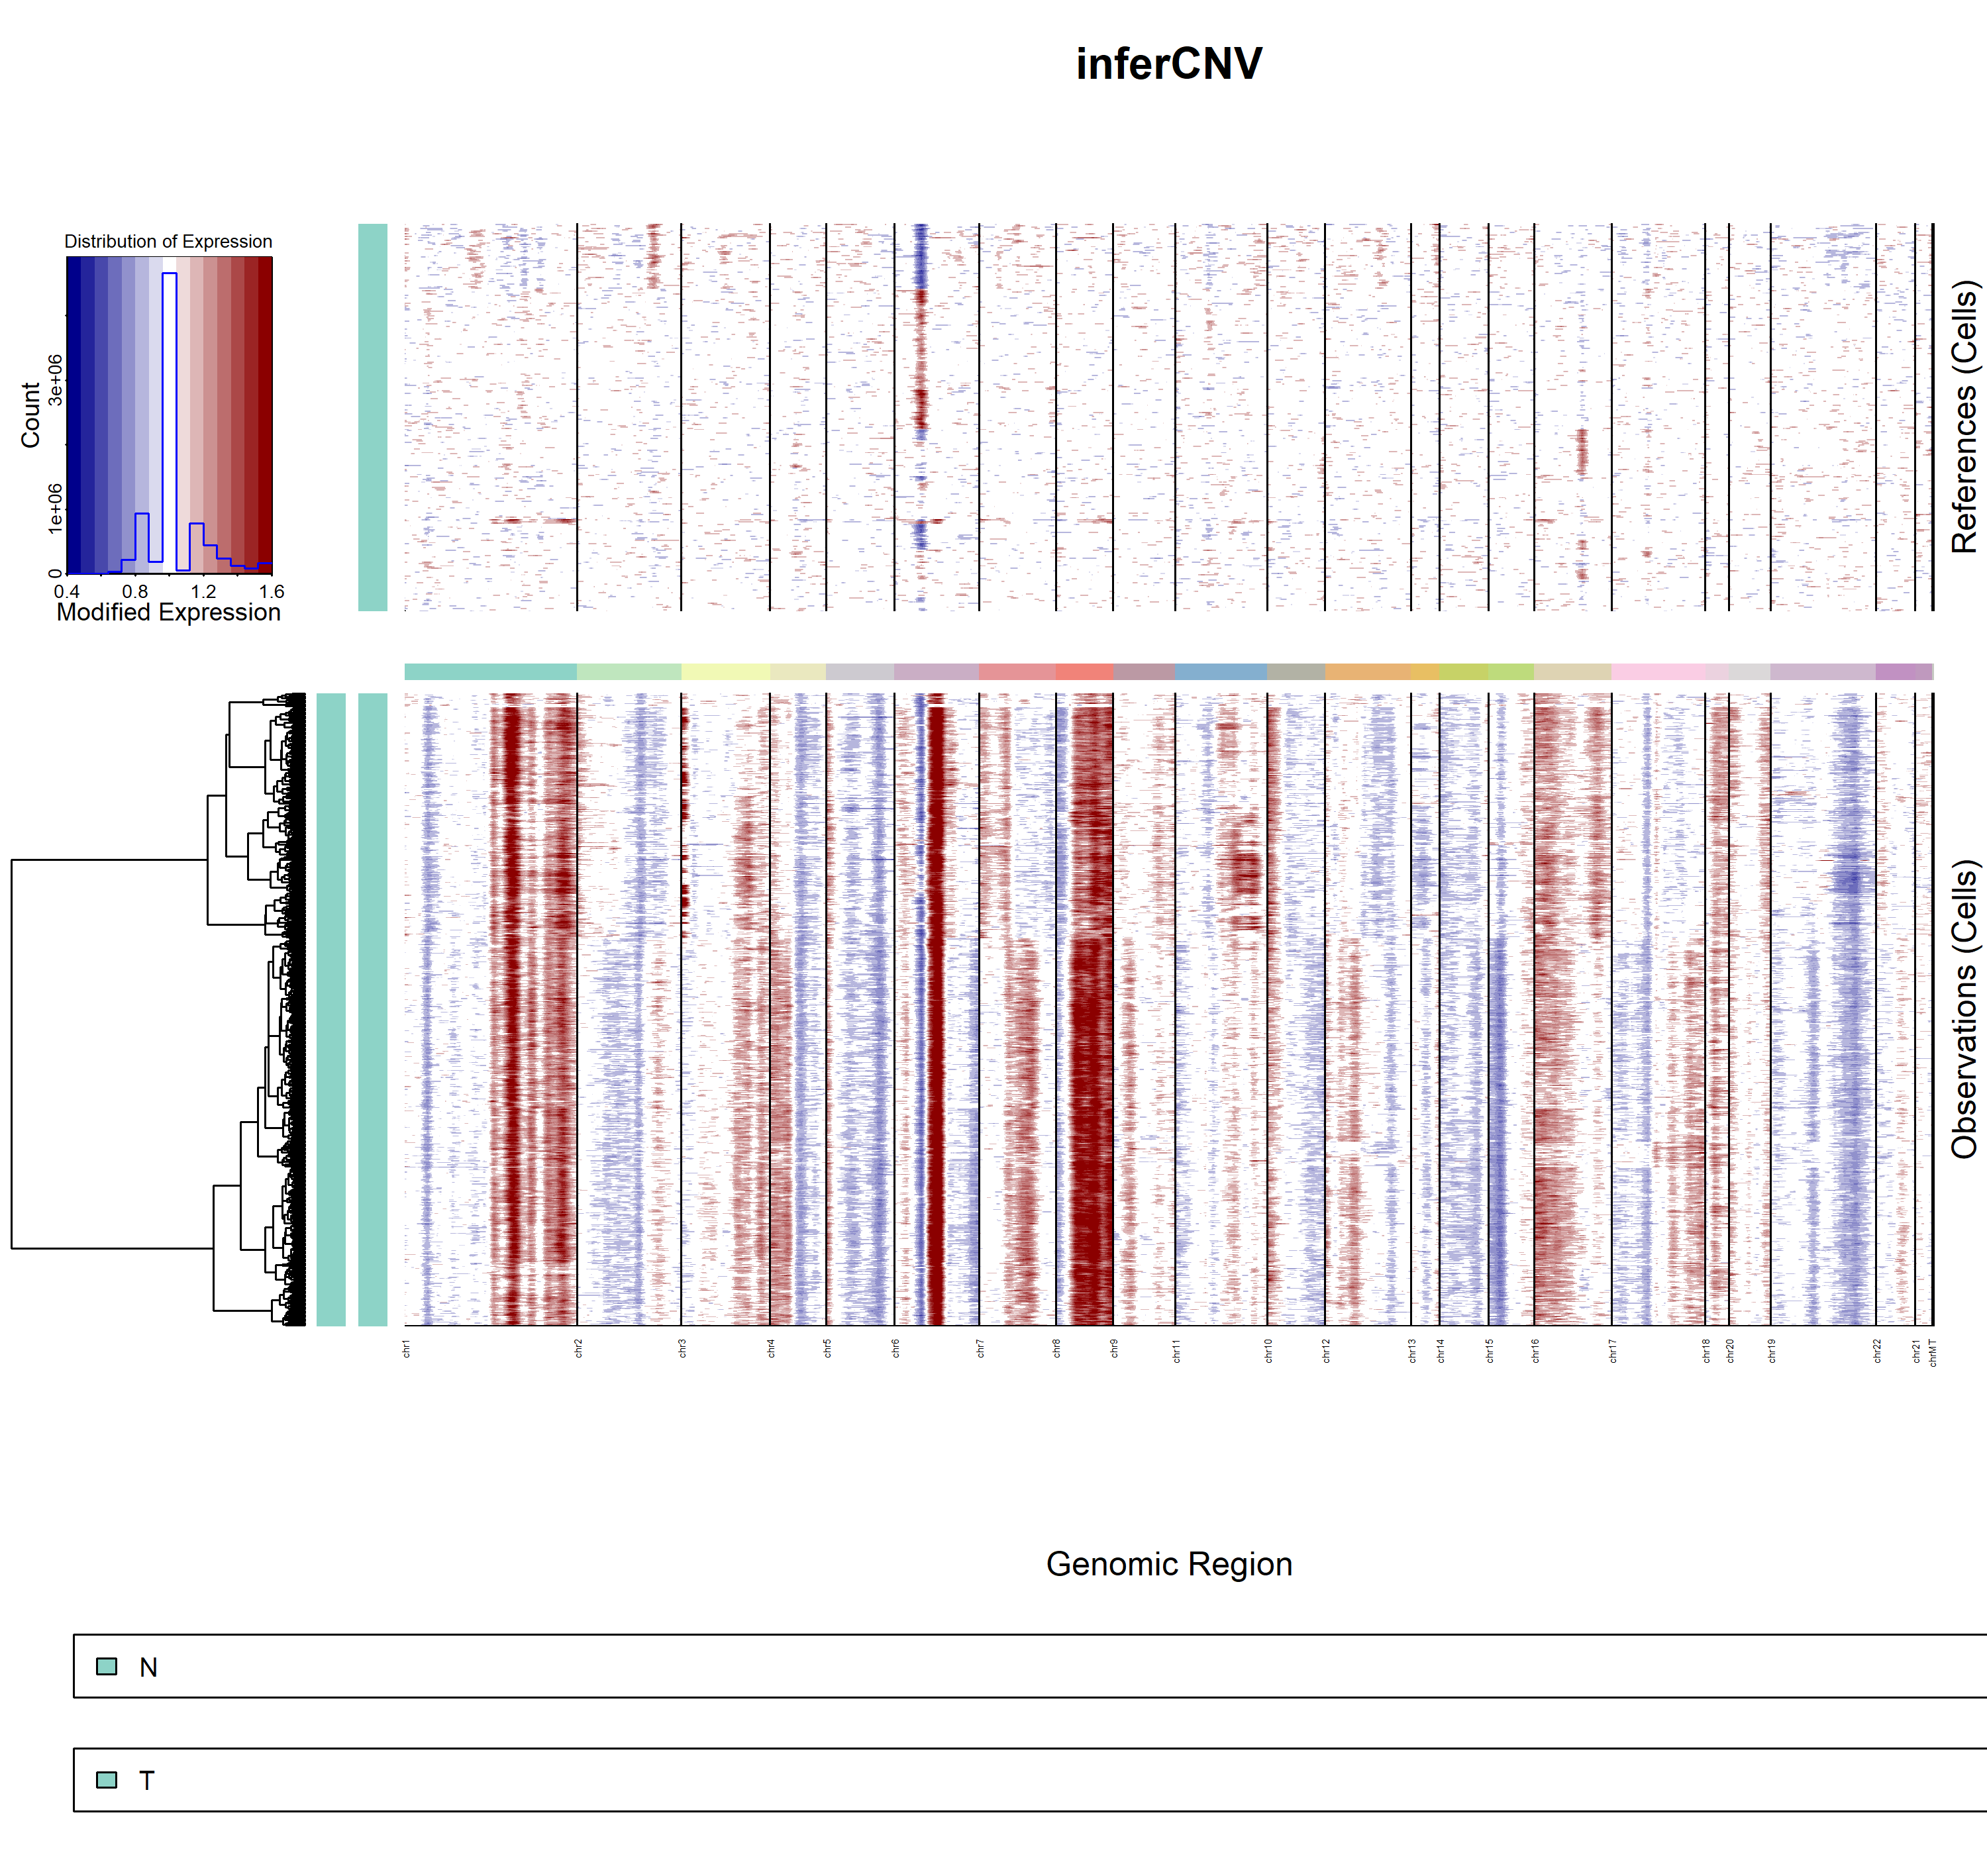
\includegraphics{./CNV_analysis_file/figs/tnbc1_demo1/infercnv.png}
\caption{infercnv1}
\end{figure}

\begin{figure}
\centering
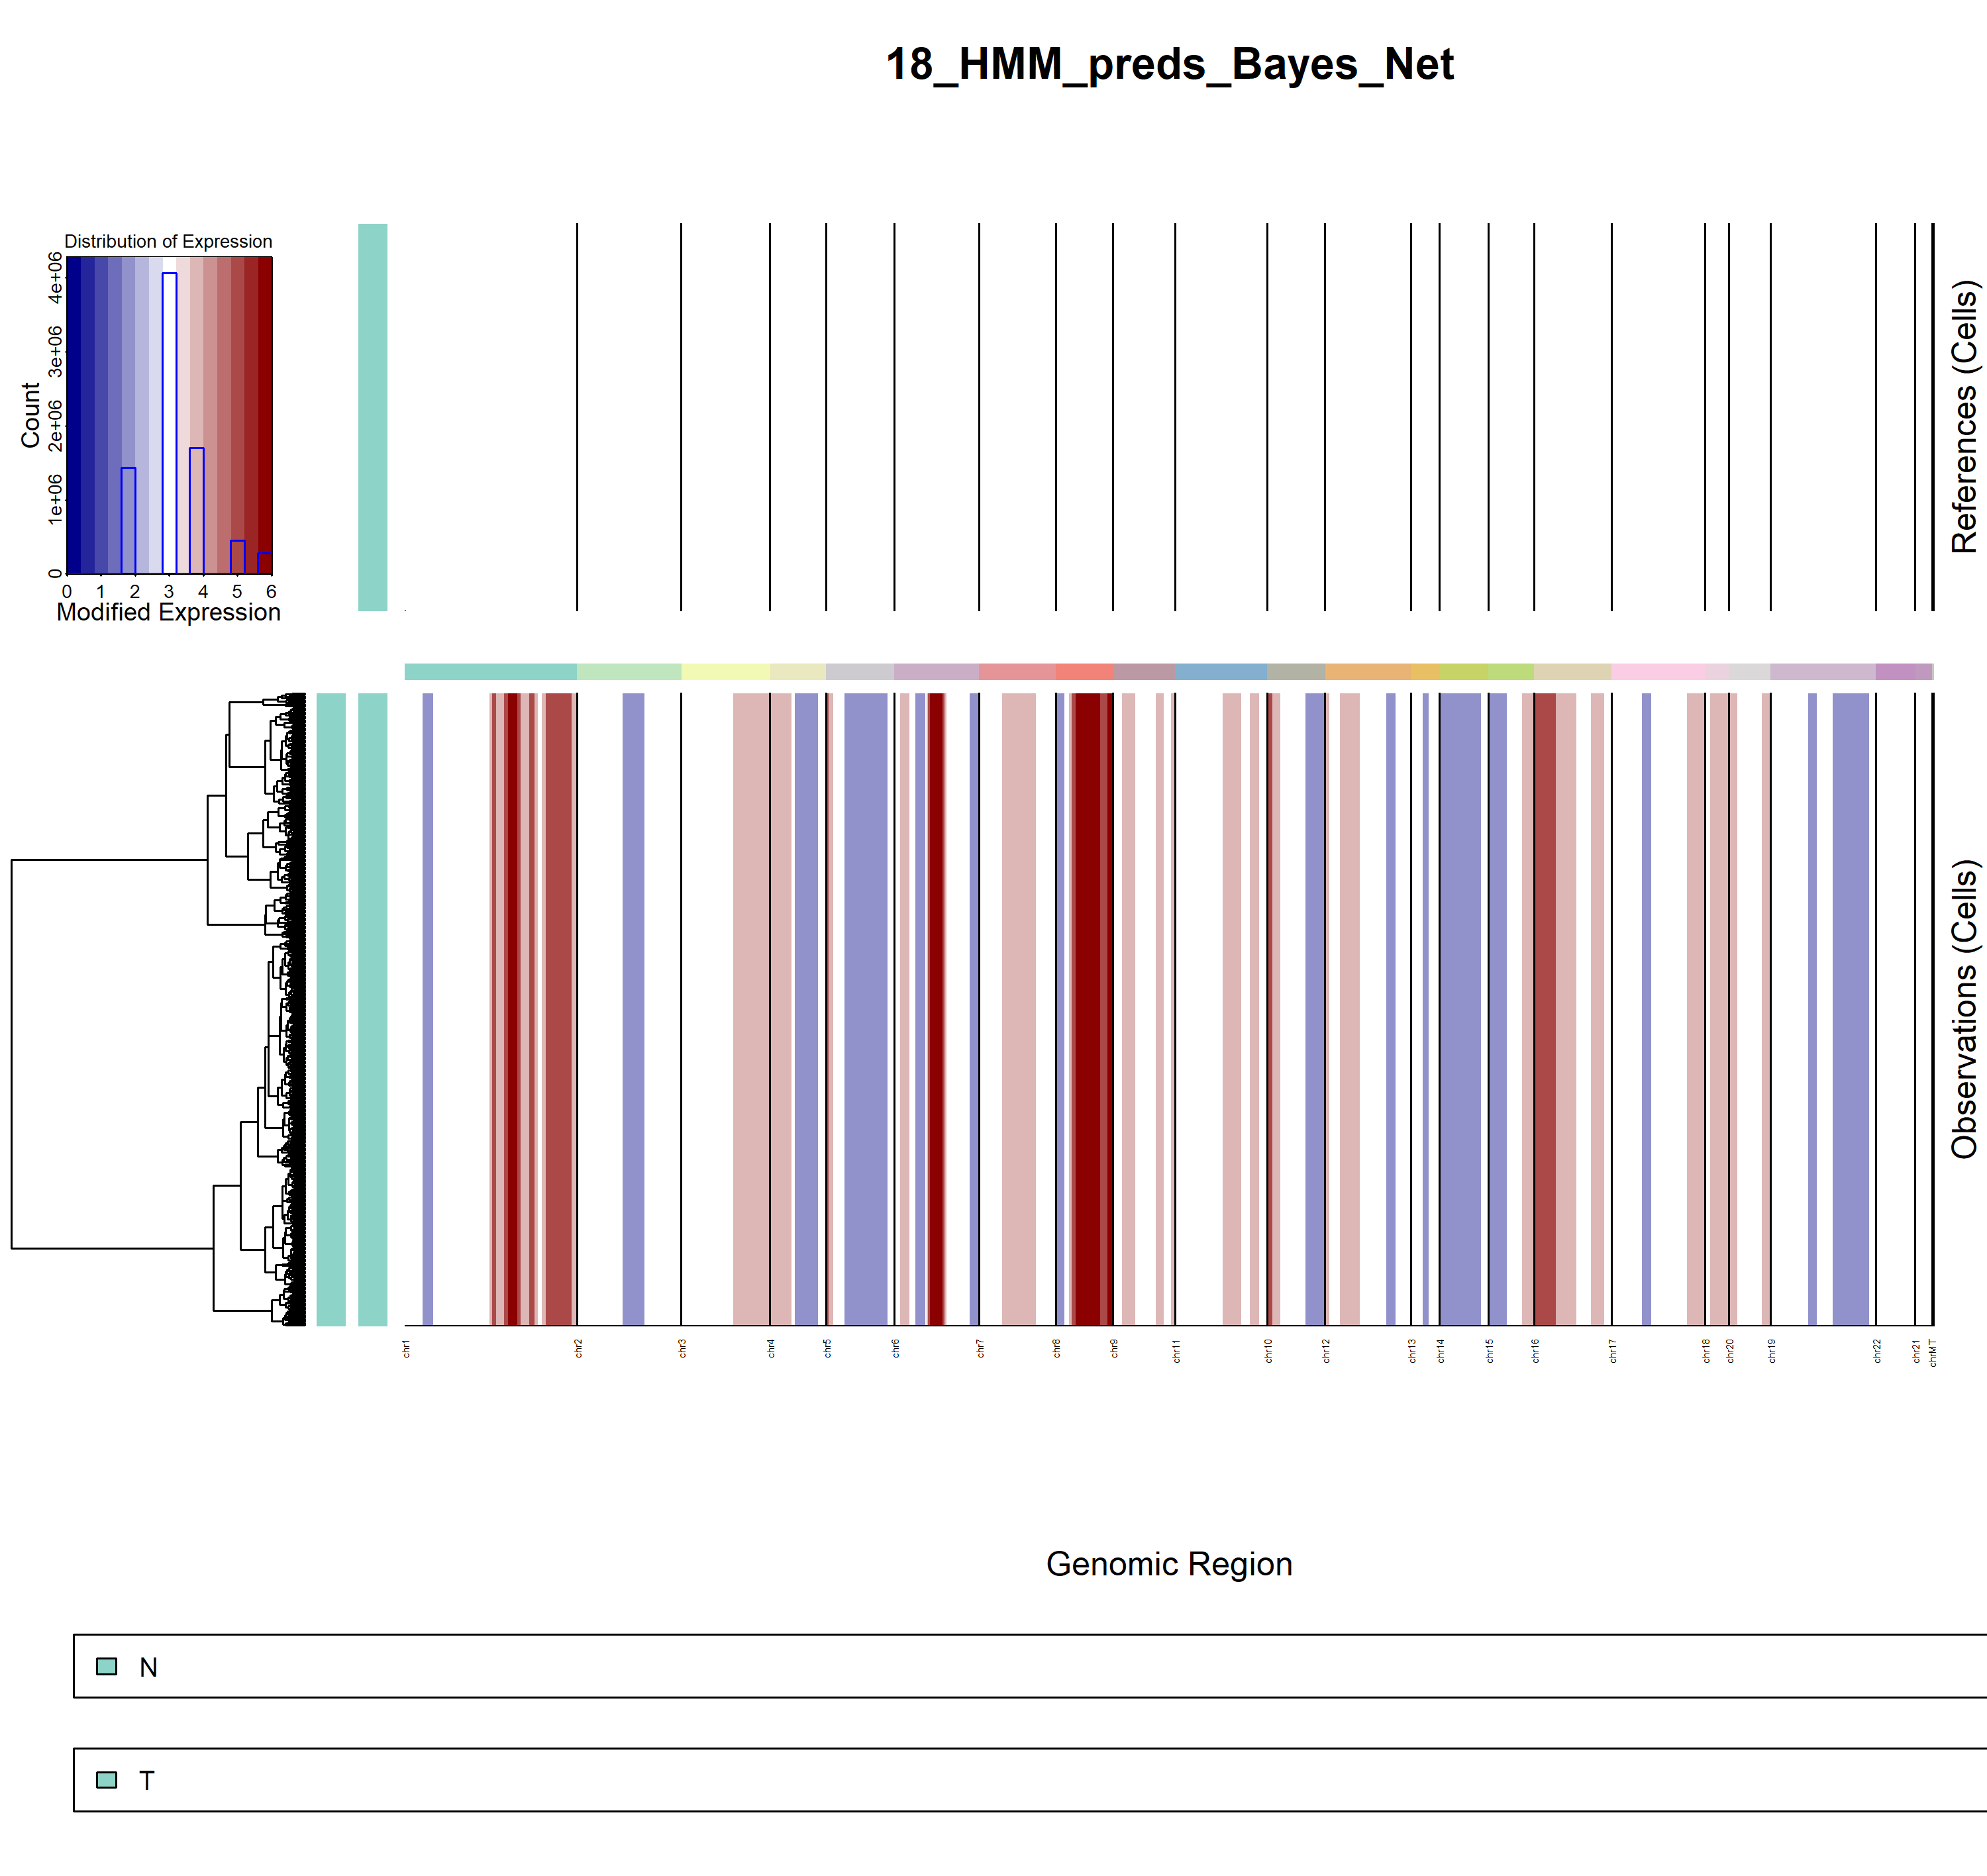
\includegraphics{./CNV_analysis_file/figs/tnbc1_demo1/infercnv.18_HMM_pred.Bayes_Net.Pnorm_0.5.png}
\caption{infercnv2}
\end{figure}

\begin{itemize}
\tightlist
\item
  demo2
\end{itemize}

\begin{figure}
\centering
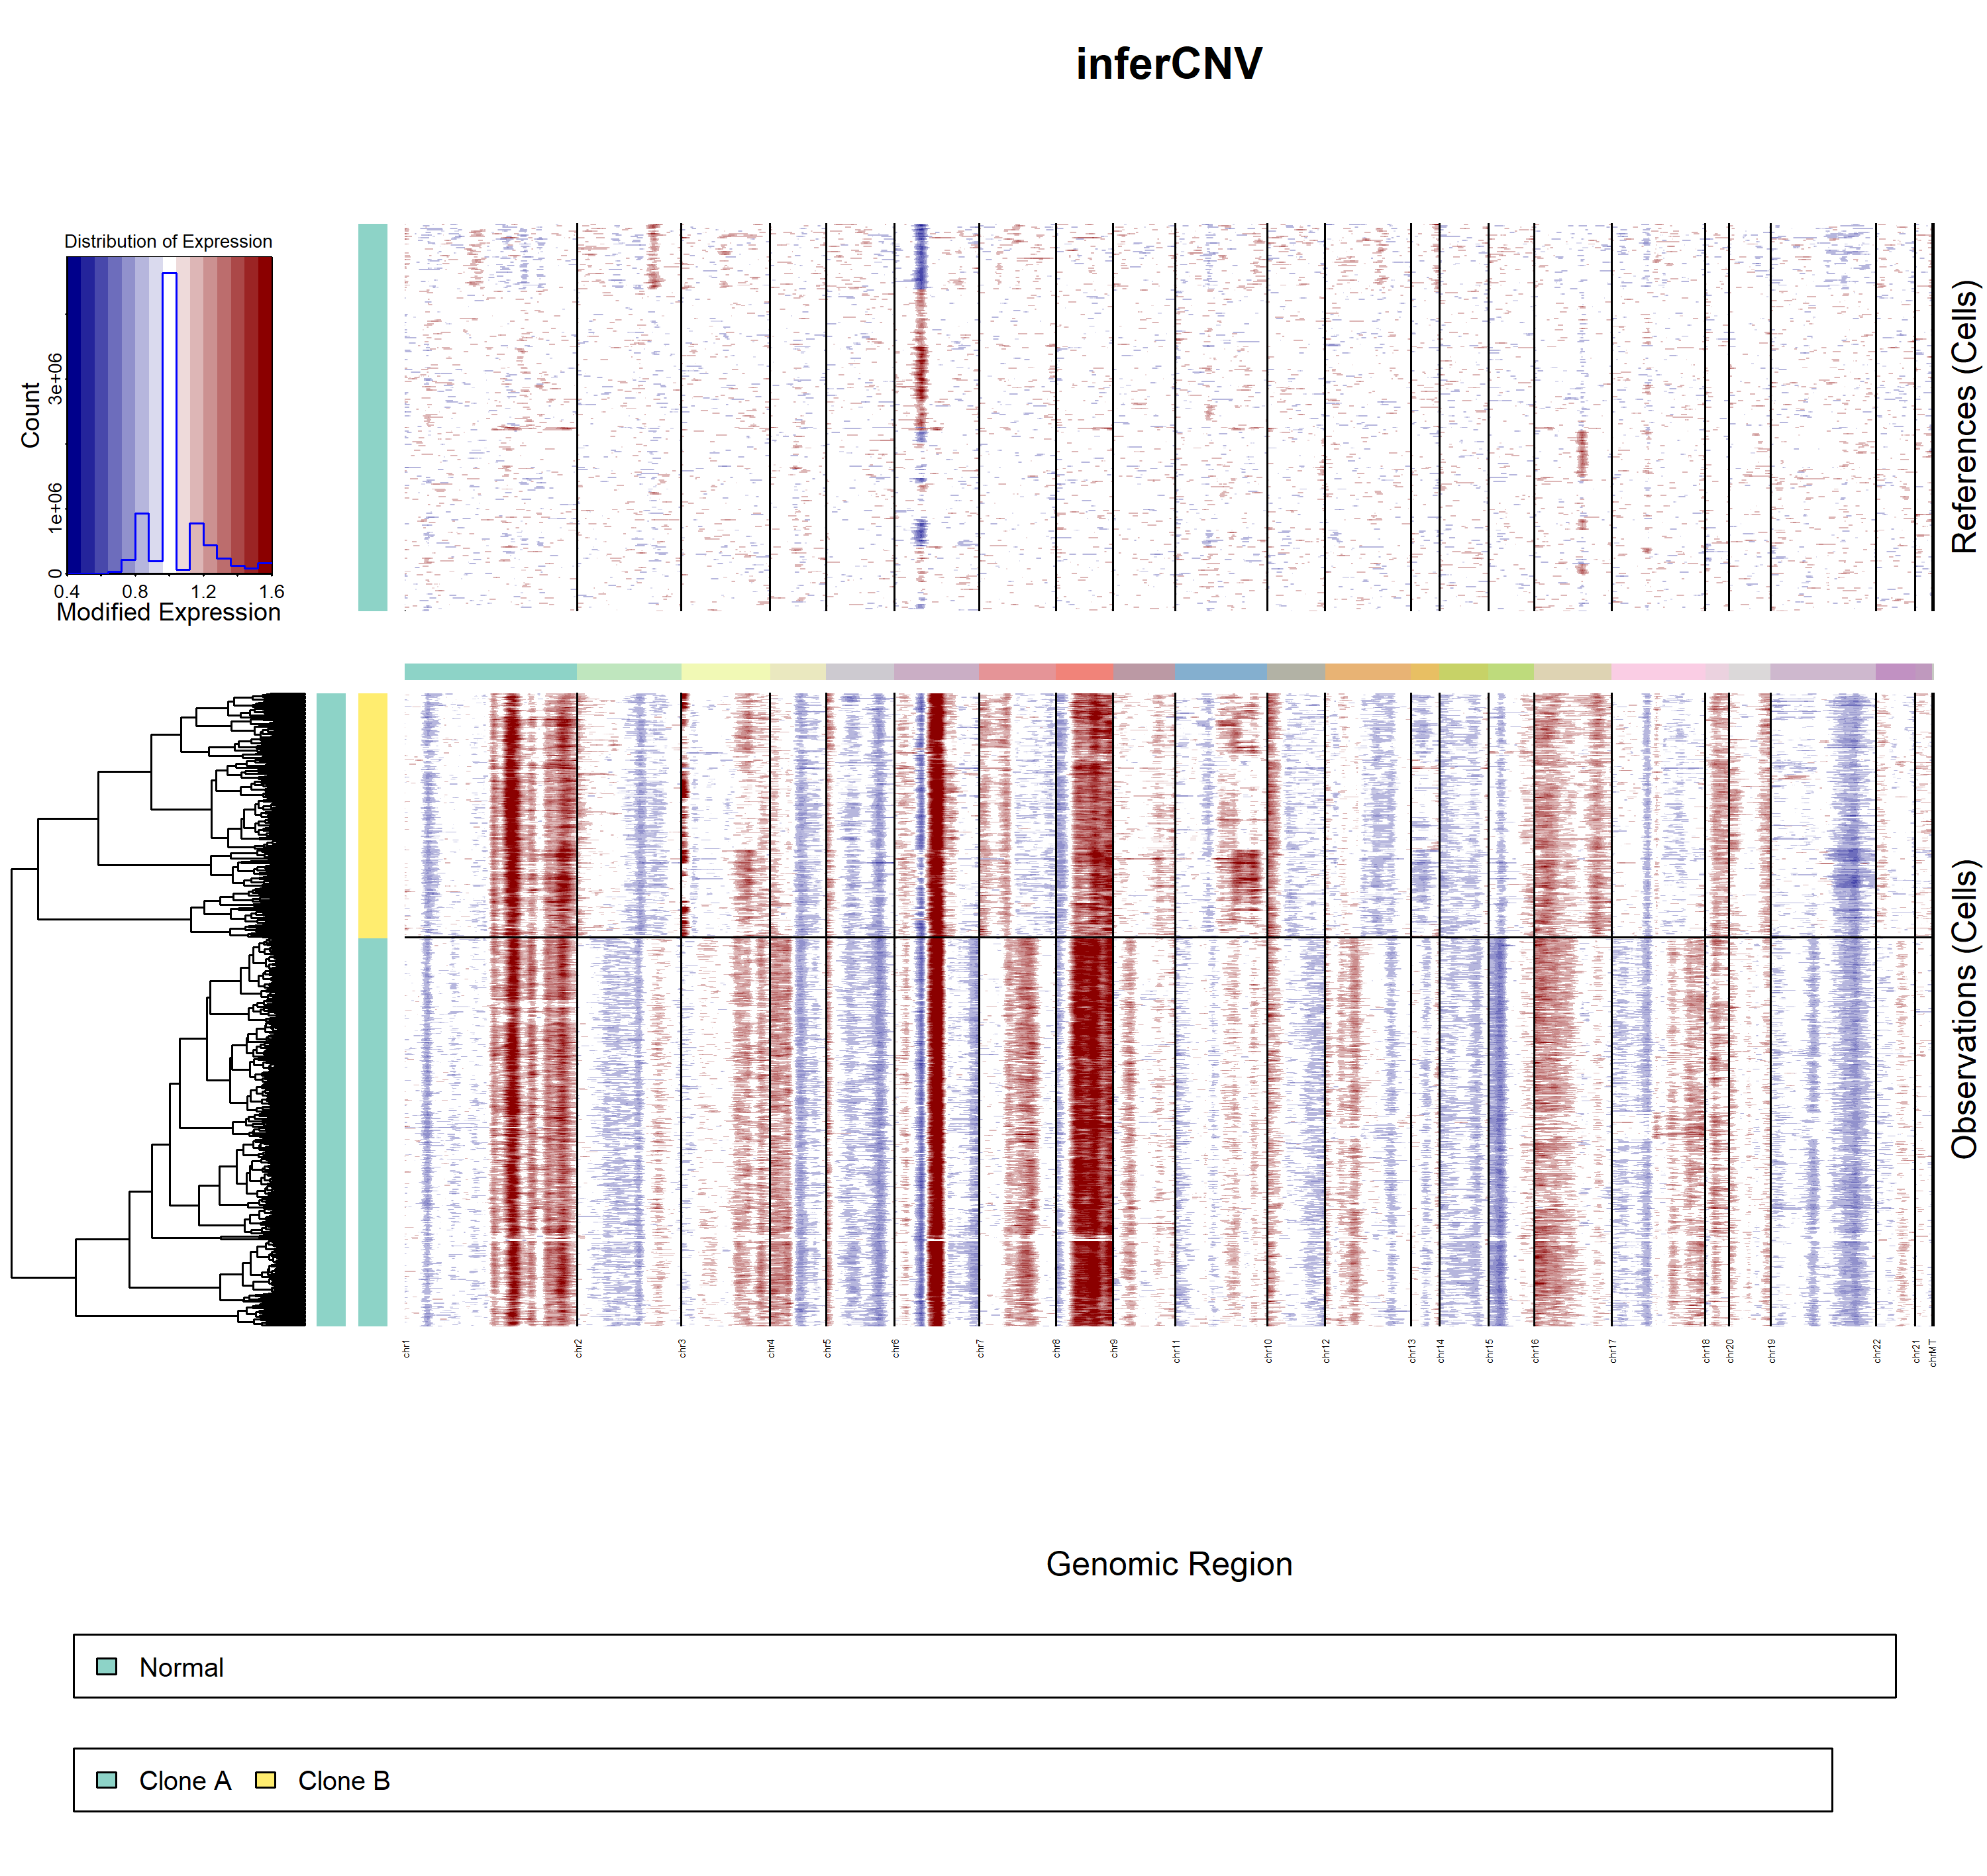
\includegraphics{./CNV_analysis_file/figs/tnbc1_demo2/infercnv.png}
\caption{infercnv3}
\end{figure}

\begin{figure}
\centering
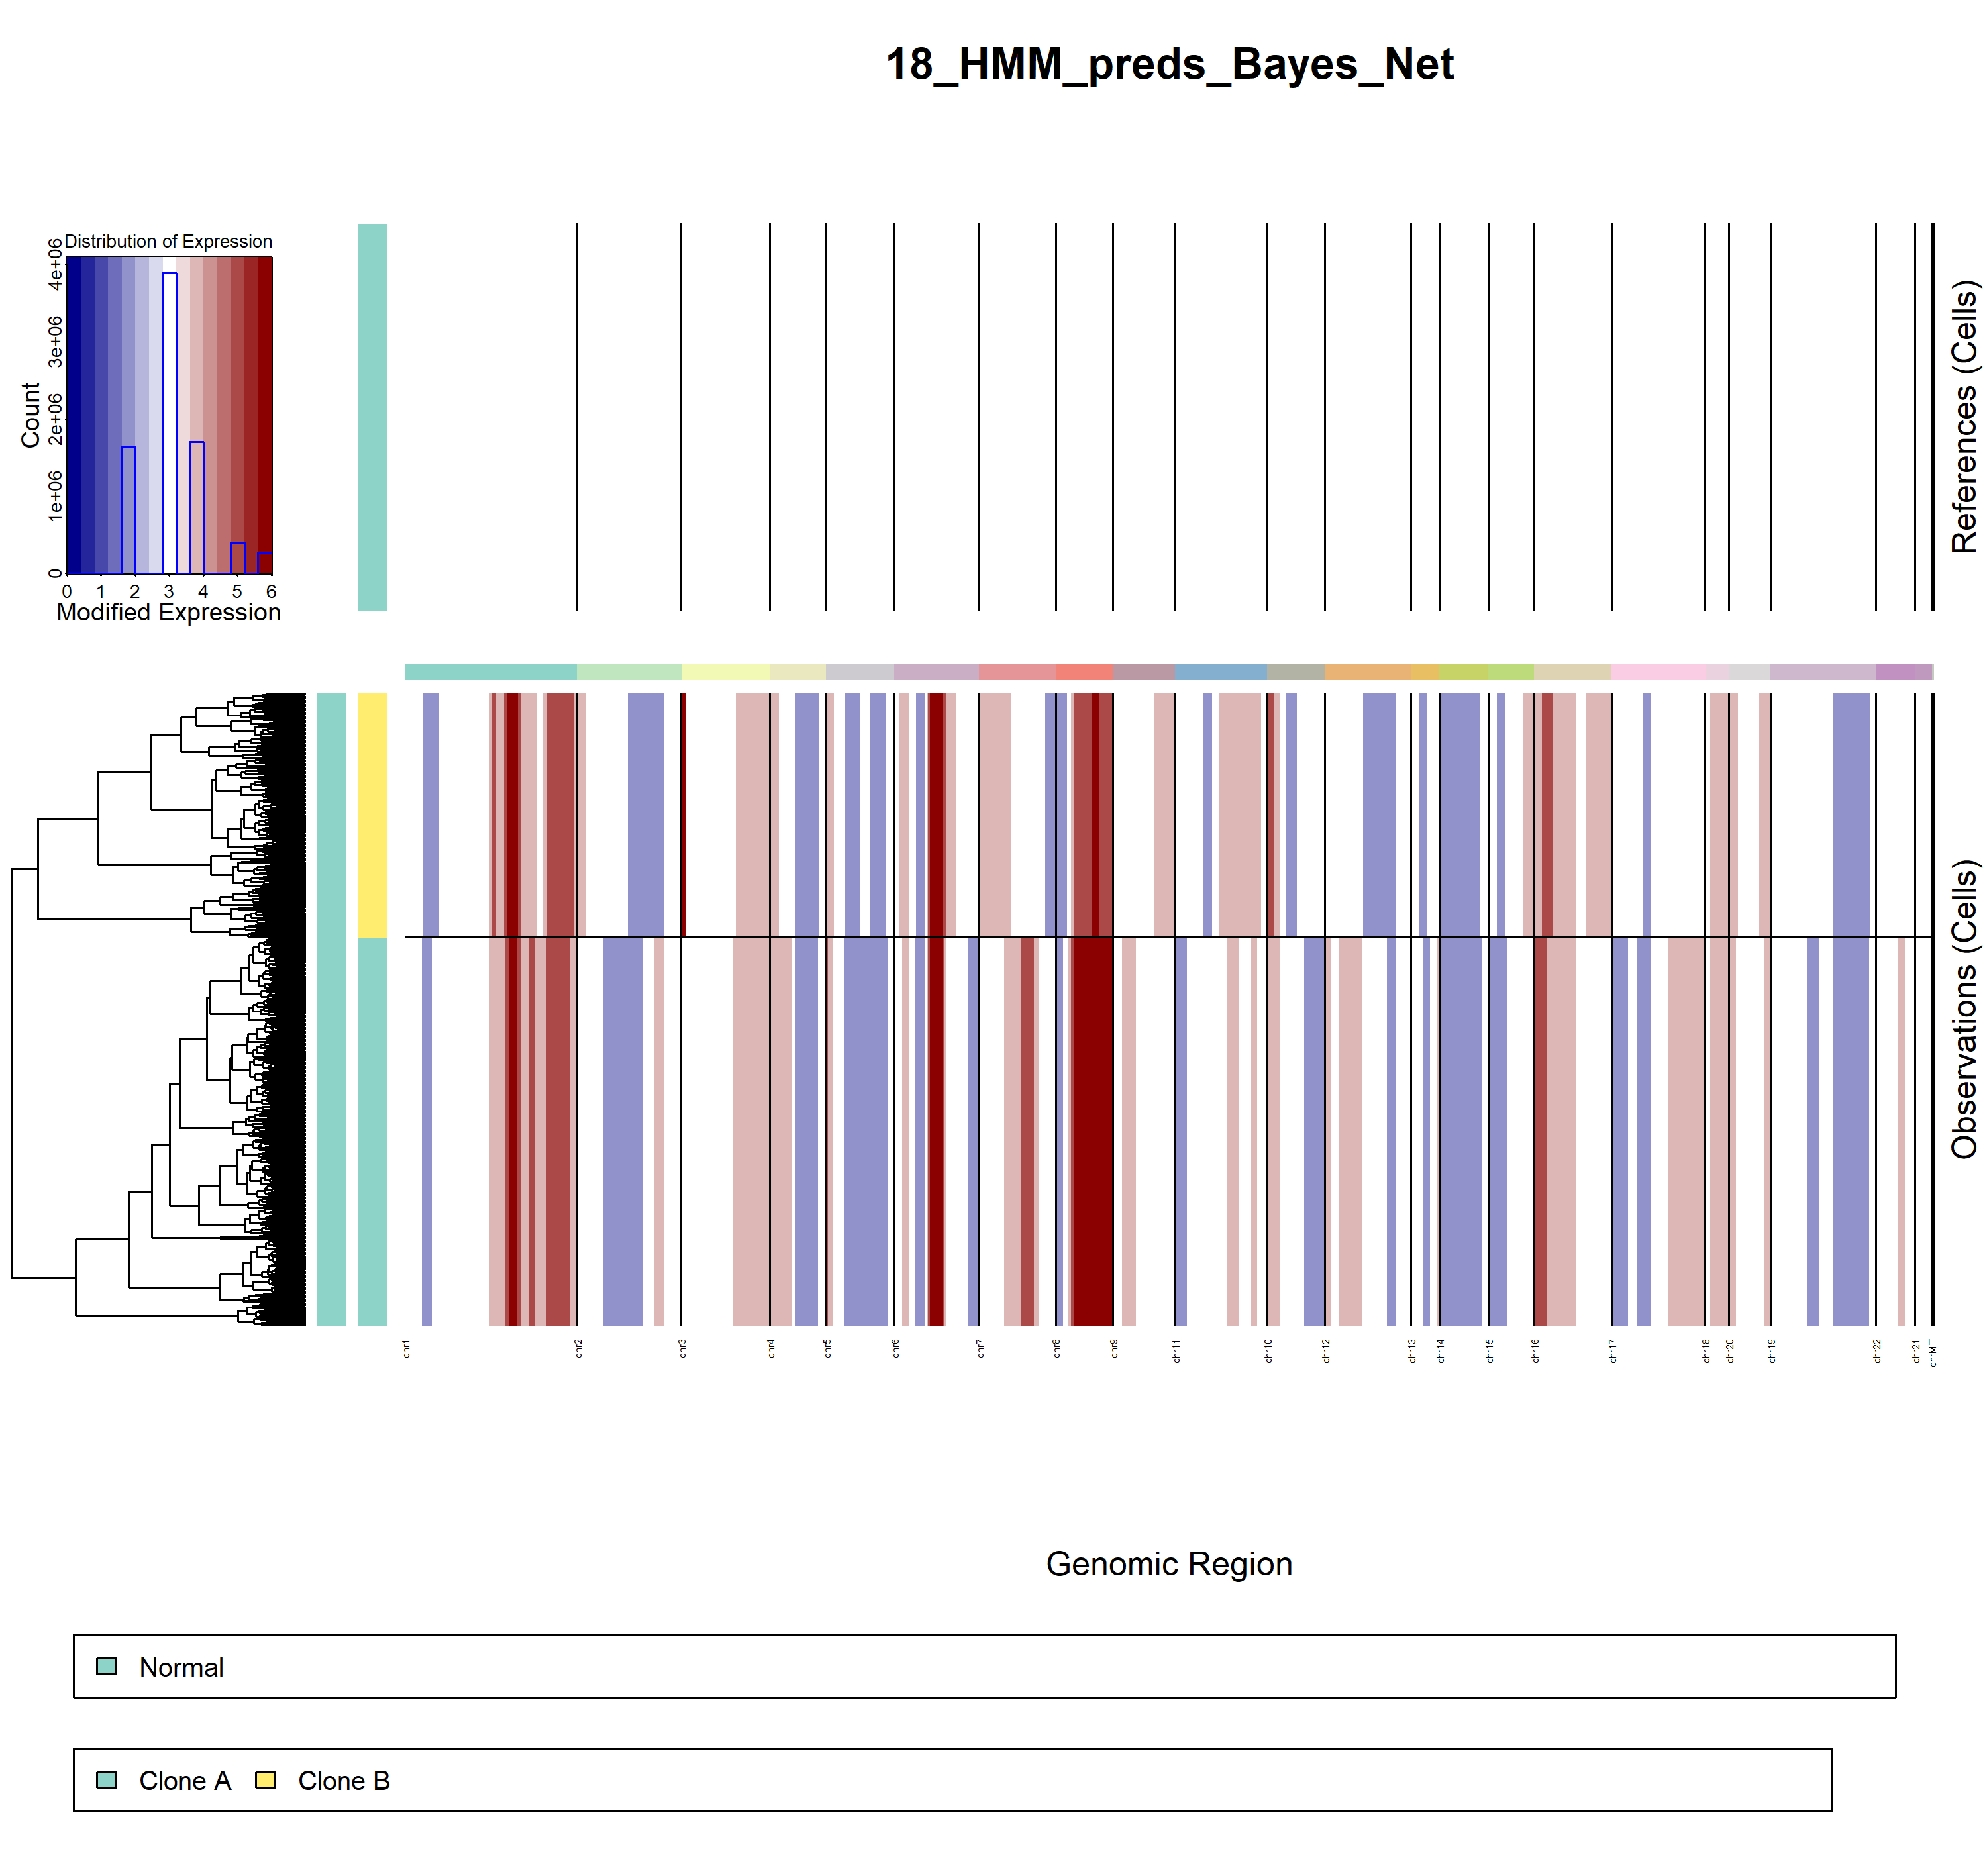
\includegraphics{./CNV_analysis_file/figs/tnbc1_demo2/infercnv.18_HMM_pred.Bayes_Net.Pnorm_0.5.png}
\caption{infercnv4}
\end{figure}

\hypertarget{ref}{%
\section{ref}\label{ref}}

\url{https://www.r-bloggers.com/2012/04/getting-started-with-jags-rjags-and-bayesian-modelling/}

\begin{verbatim}
bookdown::render_book("index.Rmd", "bookdown::gitbook")
\end{verbatim}

\hypertarget{mtdna-variants-for-lineage-inference-from-single-cell-omics}{%
\chapter{mtDNA variants for lineage inference from single-cell omics}\label{mtdna-variants-for-lineage-inference-from-single-cell-omics}}

\hypertarget{pileup-with-cellsnp-lite}{%
\section{Pileup with cellsnp-lite}\label{pileup-with-cellsnp-lite}}

Cellsnp-lite is designed to perform efficient pileup and genotyping for both bulk and single cell sequencing data. It could be easily installed via \protect\hyperlink{conda_install}{conda} with \texttt{conda\ install\ -c\ bioconda\ -c\ conda-forge\ cellsnp-lite}.

In this example, we use cellsnp-lite to pileup chrM on a SMART-seq2 dataset, whose output could be used as inputs of MQuad model for mitochondrial clone analysis.

\textbf{Note that we have uploaded the pileup results of cellsnp-lite to \href{https://sourceforge.net/projects/sgcellworkshop/files/mtDNA_analysis/}{sgcellworkshop} repo on sourceforge. You can directly download the \texttt{joxm.hg19.cellsnp.mode2b.tar.gz} file and then run \texttt{tar\ zxvf\ joxm.hg19.cellsnp.mode2b.tar.gz} to unpack it.}

If you want to repeat the pileup processing, please follow the steps below.

\begin{itemize}
\tightlist
\item
  Step 1. Download the bam files
\end{itemize}

The 77 SMART-seq2 bam files (\textasciitilde3.5G) were packed into one file \texttt{joxm.bam.all.77.tar.gz}. This file, together with another two files \texttt{joxm.hg19.bam.lst} and \texttt{joxm.sample.lst}, should be downloaded from \href{https://sourceforge.net/projects/sgcellworkshop/files/mtDNA_analysis/}{sgcellworkshop} repo on sourceforge. Please put the three files in the same directory.

\begin{itemize}
\tightlist
\item
  Step 2. Unpack the bam files
\end{itemize}

Unpack the bam files with \texttt{tar\ zxvf\ joxm.bam.all.77.tar.gz}. The bam files, together with the \texttt{.bai} files, should be in the \texttt{sort/} directory.

\begin{itemize}
\tightlist
\item
  Step 3. Run cellsnp-lite
\end{itemize}

\begin{verbatim}
cellsnp-lite      \
  -S ./joxm.hg19.bam.lst    \
  -i ./joxm.sample.lst      \
  -O ./cellsnp              \
  --chrom MT        \
  --cellTAG None    \
  --UMItag None     \
  --minCOUNT 20     \
  --minMAF 0        \
  --genotype        \
  --gzip
\end{verbatim}

\hypertarget{clonal-analysis-with-mquad}{%
\section{Clonal analysis with MQuad}\label{clonal-analysis-with-mquad}}

We have finished a nice book.

  \bibliography{book.bib,packages.bib}

\end{document}
